\chapter{Experiments} \label{ch:experiments}

\section{Localization evaluation}
We evaluate the five \acrshort{wsol} methods that are described in detail in section \ref{lb:wsol_methods}: CAM, Grad-CAM, Grad-CAM++, Score-CAM and MinMaxCAM. All these methods are evaluated using a VGG-GAP network and a ResNet-50 network, except for Grad-CAM, which is a generalization of CAM that yields the same score maps as CAM in a \acrshort{cnn} with a \acrshort{gap} layer like the VGG16-GAP and ResNet-50 networks. Grad-CAM, Grad-CAM++ and Score-CAM are also evaluated using a VGG16 network. As these methods don't require an architecture with \acrshort{gap} layer, it is interesting to see how they perform on the unmodified VGG16 architecture.

The localization methods are evaluated for the mentioned networks on the synthetic datasets and on the ImageNet dataset. For the VGG16-GAP network and the ResNet-50 network, we trained two models per network on the datasets: One without regularization and one with MinMaxCAM regularization. The localization methods CAM, Grad-CAM++ and Score-CAM are evaluated on both models. For the VGG16 network we only train one model without regularization per synthetic dataset as MinMaxCAM is not compatible with this network. 

\subsection{Synthetic datasets}
We evaluate the \acrshort{cam}-based family of localization methods on the synthetic datasets listed in Table \ref{tab:synthetic_datasets}, using the MaxBoxAccV3 precision and recall metrics, and the \acrshort{pxap} metric. In following sections, results for VGG16-GAP, VGG16 and ResNet-50 architectures are discussed.

\subsubsection{VGG16-GAP}
The localization results using the multiple-instance \acrshort{wsol} metrics MaxBoxAccV3 recall and precision are shown in Table \ref{tab:maxboxaccv3_recall_vgg16_gap_synthetic} and Table \ref{tab:maxboxaccv3_precision_vgg16_gap_synthetic}. The pixel average precision results are illustrated in Table \ref{tab:pxap_vgg16_gap_synthetic}. 

\begin{table}[h]
\centering
\begin{tabular}{lrrrrrrrr}
\toprule
& \multicolumn{8}{c}{VGG16-GAP synthetic (MaxBoxAccV3 recall)} \\
method & d1b & d1t & d2b & d2t & d3b & d3t & d4b & d4t \\
\cmidrule(lr){1-1} \cmidrule(lr){2-9} 
CAM & \color{purple} \bfseries  \underline{91.50} & \color{teal} \bfseries 91.17 & \color{purple} \bfseries 67.33 & \color{purple} \bfseries 66.92 & \color{purple} \bfseries 59.33 & 58.33 & \color{purple} \bfseries \underline{48.58} & 54.00 \\
Grad-CAM++ & 92.67 & 90.67 & 68.50 & 67.75 & 60.17 & \color{purple} \bfseries 57.83 & 49.12 & \color{purple} \bfseries 53.04 \\
Score-CAM & \color{teal} \bfseries 92.83 & \color{purple} \bfseries \underline{90.17} & \color{teal} \bfseries 72.83 & \color{teal} \bfseries 69.42 & \color{teal} \bfseries \underline{64.89} & \color{teal} \bfseries \underline{61.33} & \color{teal} \bfseries 53.25 & \color{teal} \bfseries 55.67 \\
\cmidrule(lr){1-1} \cmidrule(lr){2-9} 
MinMaxCAM & \color{purple} \bfseries 91.67 & \color{purple} \bfseries 92.00 & \color{purple} \bfseries \underline{67.00} & \color{purple} \bfseries \underline{66.33} & \color{purple} \bfseries \underline{59.11} & \color{purple} \bfseries \underline{57.17} & \color{purple} \bfseries 53.25 & \color{purple} \bfseries \underline{47.67} \\
Grad-CAM++ & 94.17 & \color{teal} \bfseries \underline{93.67} & 67.50 & 67.00 & 59.94 & 57.17 & 54.46 & 49.62 \\
Score-CAM & \color{teal} \bfseries \underline{95.00} & 93.50 & \color{teal} \bfseries \underline{73.75} & \color{teal} \bfseries \underline{70.83} & \color{teal} \bfseries 64.83 & \color{teal} \bfseries 61.22 & \color{teal} \bfseries \underline{61.37} & \color{teal} \bfseries \underline{57.96} \\
\bottomrule
\end{tabular}
\caption[MaxBoxAccV3 recall for VGG16-GAP on synthetic datasets]{MaxBoxAccV3 recall for VGG16-GAP on synthetic datasets. First 3 rows show evaluation results for CAM-based methods evaluated on the non-regularized model. Last 3 rows show results for CAM-based models evaluated on MinMaxCAM-regularized model. Column-wise minimum and maximum per sub-table are highlighted in red and green. Global column-wise minimum and maximum are underlined.}
\label{tab:maxboxaccv3_recall_vgg16_gap_synthetic}
\end{table}

\begin{table}[h]
\centering
\begin{tabular}{lrrrrrrrr}
\toprule
 & \multicolumn{8}{c}{VGG16-GAP synthetic (MaxBoxAccV3 precision)} \\
method & d1b & d1t & d2b & d2t & d3b & d3t & d4b & d4t \\
\cmidrule(lr){1-1} \cmidrule(lr){2-9} 
CAM & 85.16 & 85.78 & \color{purple} \bfseries 72.72 & \color{purple} \bfseries 71.52 & 67.91 & 65.07 & 59.15 & 63.10 \\
Grad-CAM++ & \color{teal} \bfseries 85.95 & \color{teal} \bfseries 85.97 & 73.27 & 71.69 & \color{purple} \bfseries 67.08 & \color{purple} \bfseries \underline{64.03} & \color{purple} \bfseries \underline{58.24} & \color{purple} \bfseries 61.36 \\
Score-CAM & \color{purple} \bfseries \underline{84.91} & \color{purple} \bfseries \underline{83.40} & \color{teal} \bfseries 75.42 & \color{teal} \bfseries 72.33 & \color{teal} \bfseries \underline{70.46} & \color{teal} \bfseries 66.94 & \color{teal} \bfseries 61.62 & \color{teal} \bfseries 63.35 \\
\cmidrule(lr){1-1} \cmidrule(lr){2-9} 
MinMaxCAM & \color{purple} \bfseries 86.26 & \color{purple} \bfseries 86.54 & 71.76 & 70.90 & 67.23 & 66.16 & 65.96 & \color{purple} \bfseries \underline{57.56} \\
Grad-CAM++ & \color{teal} \bfseries \underline{89.84} & \color{teal} \bfseries \underline{89.73} & \color{purple} \bfseries \underline{71.59} & \color{purple} \bfseries \underline{70.82} & \color{purple} \bfseries \underline{66.45} & \color{purple} \bfseries 65.97 & \color{purple} \bfseries 64.54 & 58.59 \\
Score-CAM & 88.40 & 88.28 & \color{teal} \bfseries \underline{76.38} & \color{teal} \bfseries \underline{72.84} & \color{teal} \bfseries 70.22 & \color{teal} \bfseries \underline{67.07} & \color{teal} \bfseries \underline{68.30} & \color{teal} \bfseries \underline{65.22} \\
\bottomrule
\end{tabular}
\caption[MaxBoxAccV3 for VGG16-GAP on synthetic datasets]{MaxBoxAccV3 precision for VGG16-GAP on synthetic datasets. First 3 rows show evaluation results for CAM-based methods evaluated on the non-regularized model. Last 3 rows show results for CAM-based models evaluated on MinMaxCAM-regularized model. Column-wise minimum and maximum per sub-table are highlighted in red and green. Global column-wise minimum and maximum are underlined.}
\label{tab:maxboxaccv3_precision_vgg16_gap_synthetic}
\end{table}

\begin{table}[H]
\centering
\begin{tabular}{lrrrrrrrr}
\toprule
 & \multicolumn{8}{c}{VGG16-GAP synthetic (PxAP)} \\
method & d1b & d1t & d2b & d2t & d3b & d3t & d4b & d4t \\
\cmidrule(lr){1-1} \cmidrule(lr){2-9} 
CAM & 79.89 & 83.12 & 77.41 & 78.54 & \color{purple} \bfseries \underline{74.37} & 71.37 & \color{purple} \bfseries \underline{66.02} & 71.37 \\
Grad-CAM++ & \color{teal} \bfseries 80.82 & \color{teal} \bfseries 83.81 & \color{teal} \bfseries 78.82 & \color{teal} \bfseries \underline{79.12} & \color{teal} \bfseries \underline{75.97} & \color{purple} \bfseries \underline{71.27} & 66.72 & \color{purple} \bfseries 71.22 \\
Score-CAM & \color{purple} \bfseries \underline{79.51} & \color{purple} \bfseries \underline{82.79} & \color{purple} \bfseries \underline{76.57} & \color{purple} \bfseries \underline{76.23} & 75.36 & \color{teal} \bfseries 73.06 & \color{teal} \bfseries 67.38 & \color{teal} \bfseries 72.47 \\
\cmidrule(lr){1-1} \cmidrule(lr){2-9} 
MinMaxCAM & 82.93 & \color{purple} \bfseries 82.80 & \color{purple} \bfseries 77.65 & 77.39 & \color{purple} \bfseries 74.39 & \color{purple} \bfseries 72.28 & \color{purple} \bfseries 70.91 & \color{purple} \bfseries \underline{64.78} \\
Grad-CAM++ & \color{teal} \bfseries \underline{84.13} & 84.26 & \color{teal} \bfseries \underline{79.10} & \color{teal} \bfseries 78.45 & \color{teal} \bfseries 75.76 & 72.66 & 72.93 & 68.22 \\
Score-CAM & \color{purple} \bfseries 82.83 & \color{teal} \bfseries \underline{84.65} & 77.66 & \color{purple} \bfseries 77.30 & 75.61 & \color{teal} \bfseries \underline{74.31} & \color{teal} \bfseries \underline{75.48} & \color{teal} \bfseries \underline{75.14} \\
\bottomrule
\end{tabular}
\caption[PxAP for VGG16-GAP on synthetic datasets]{PxAP for VGG16-GAP on synthetic datasets. First 3 rows show evaluation results for CAM-based methods evaluated on the non-regularized model. Last 3 rows show results for CAM-based models evaluated on MinMaxCAM-regularized model. Column-wise minimum and maximum per sub-table are highlighted in red and green. Global column-wise minimum and maximum are underlined.}
\label{tab:pxap_vgg16_gap_synthetic}
\end{table}

For each table, the first three rows represent the results using localization methods on the non-regularized model, and the next three rows show the results for the MinMaxCAM regularized model. As the MinMaxCAM method uses the same localization method as the CAM method, the latter is represented in the bottom part of the table by the MinMaxCAM method. For each sub-table the column-wise minimum and maximum value per dataset are highlighted respectively in red and green. The overall column-wise minimum and maximum values are underlined. 

From the results in Tables \ref{tab:maxboxaccv3_recall_vgg16_gap_synthetic}, \ref{tab:maxboxaccv3_precision_vgg16_gap_synthetic} and \ref{tab:pxap_vgg16_gap_synthetic} we can make following observations:

\textbf{Multi-instance localization recall and precision} decrease for datasets with increasing number of object instances, albeit that precision is decreasing less severe. MaxBoxAccV3 recall is above 90\% for the single instance datasets d1b and d1t, significantly lower for the 2-instance and 3-instance datasets and worst for the datasets with four object instances per image. It's remarkable to notice that even for the worst performing models, still around half of all object instances can be localized with a model that is trained for classification only. 

\textbf{Pixel average precision} doesn't drop as significantly as the MaxBoxAccV3 metrics for images with multiple object instances. Intuitively, a reasonable explanation is that a mismatch at pixel level causes a less severe penalty than a mismatch at the coarse-grained bounding box level.

\textbf{Score-CAM localization metrics for multi-instance datasets} are higher than metrics of other methods, with the exception for the PxAP metric where Grad-CAM++ performs better for the 2-instance dataset variants. The promising results for multi-target visualization observed by Wang \textit{et al.} \cite{wang2020score}, seem to hold in our quantitative evaluation. 

\textbf{Models without regularization and with MinMaxCAM regularization} evaluated with the CAM-based localization methods, show the same multi-instance localization performance trend for precision and recall. This means that the localization methods performing well in non-regularized models, also perform well in MinMaxCAM-regularized models.

\textbf{Discrepancy between datasets having the same number of object instances but different variant.} When we pairwise compare datasets with the same number of object instances, we see that in most cases, the b-variant (with background) shows better MaxBoxAccV3 recall than the t-variant (without background). The exception is the 4-instance dataset variants for the model trained without regularization.

The discrepancies can be explained by comparing the training classification and localization accuracy. Figure \ref{fig:loc_vs_acc_vgg16_gap_cam_synthetic}  illustrates these metrics for CAM MaxBoxAccV3 recall on the VGG16-GAP network trained without MinMaxCAM regularization. Pair-wise comparison of MaxBoxAccV3 recall for datasets with same number of object instances, indicates that datasets having images with background show higher recall, except for d4b and d4t. Here we can see that localization recall for d4b decreases towards the later training epochs.

\begin{figure}[h]
    \begin{center}       
    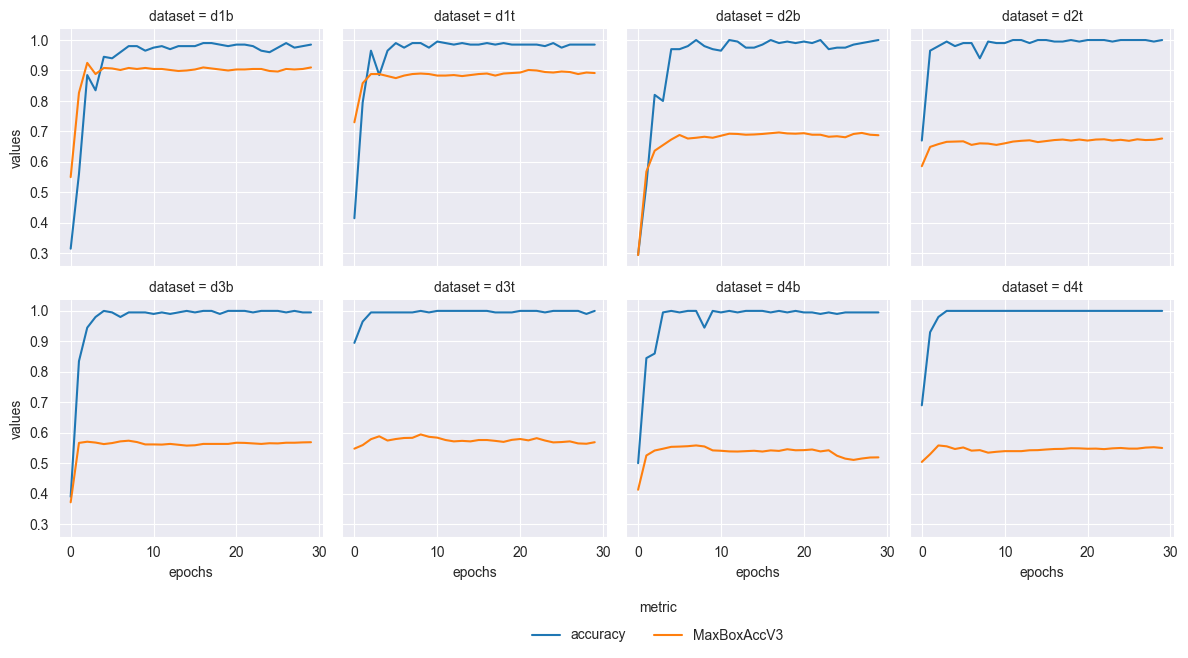
\includegraphics[width=\textwidth]{fig_loc_vs_acc_vgg16_gap_cam_synthetic.png}
    \caption[Classification versus CAM localization accuracy on VGG16-GAP for synthetic datasets]{Classification versus CAM localization accuracy on VGG16-GAP for synthetic datasets.}
    \caption*{Source: Author}
    \label{fig:loc_vs_acc_vgg16_gap_cam_synthetic}
    \end{center}
\end{figure}

Figure \ref{fig:loc_vs_acc_vgg16_gap_minmaxcam_synthetic} shows training classification and CAM MaxBoxAccV3 recall for model fine-tuned with MinMaxCAM regularization on the different datasets. Here, we observe that, except for single instance dataset, models trained for the t-variant datasets show a curve with decreasing MaxBoxAccV3 recall at later training epochs. This is in line with results in Table \ref{tab:maxboxaccv3_recall_vgg16_gap_synthetic}. As Wang \textit{et al.} \cite{wang2021minmaxcam} set out, the condition for common region regularization to work, is that a set of images for the same class should have different backgrounds. This clearly is not the case for the t-variant datasets.

\begin{figure}[ht]
    \begin{center}       
    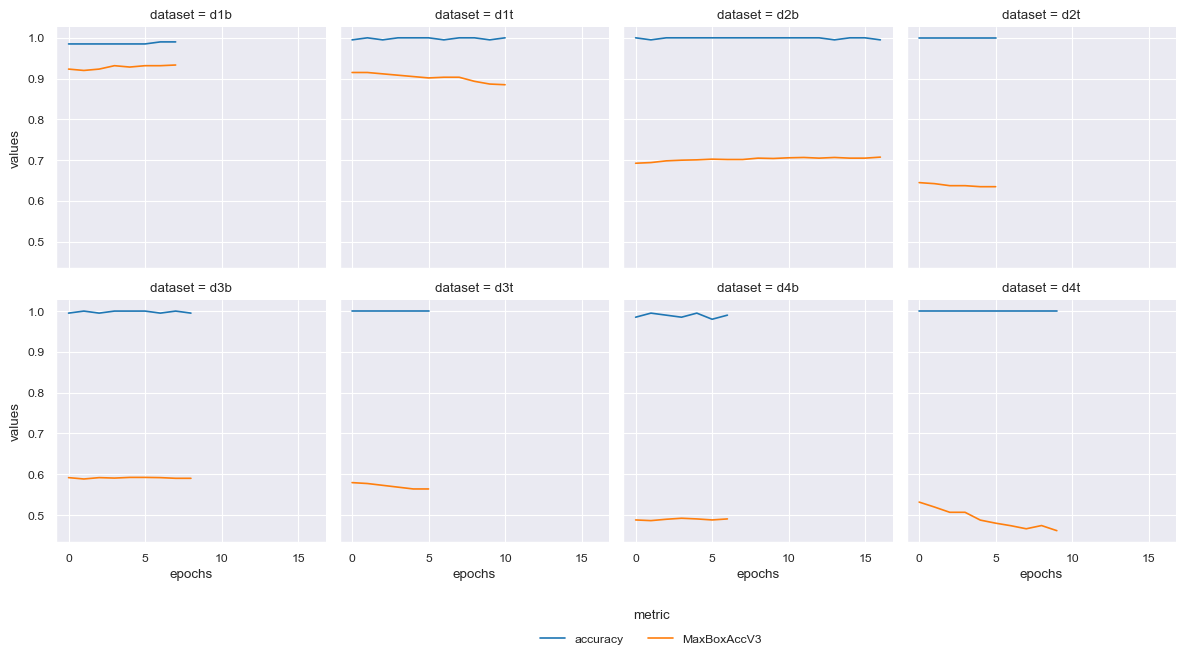
\includegraphics[width=\textwidth]{fig_loc_vs_acc_vgg16_gap_minmaxcam_synthetic.png}
    \caption[Classification versus MinMaxCAM localization accuracy on VGG16-GAP for synthetic datasets]{Classification versus MinMaxCAM localization accuracy on VGG16-GAP for synthetic datasets.}
    \caption*{Source: Author}
    \label{fig:loc_vs_acc_vgg16_gap_minmaxcam_synthetic}
    \end{center}
\end{figure}

\subsubsection{VGG16}
The localization results for VGG16 on the synthetic datasets are shown in Table \ref{tab:maxboxaccv3_recall_vgg16_base_synthetic} for MaxBoxAccV3 recall, in Table \ref{tab:maxboxaccv3_precision_vgg16_base_synthetic} for MaxBoxAccV3 precision, and in Table \ref{tab:pxap_vgg16_base_synthetic} for the PxAP metric. Note that CAM and MinMaxCAM methods cannot be used on VGG16 as this architecture has no \acrshort{gap} layer. Grad-CAM is used here as generalization of CAM.

\begin{table}[h]
\centering
\begin{tabular}{lrrrrrrrr}
\toprule
 & \multicolumn{8}{c}{VGG16 synthetic (MaxBoxAccV3 recall)} \\
method & d1b & d1t & d2b & d2t & d3b & d3t & d4b & d4t \\
\cmidrule(lr){1-1} \cmidrule(lr){2-9} 
Grad-CAM & \color{teal} \bfseries 81.33 & 68.83 & 51.17 & 46.08 & 46.94 & 45.06 & 45.33 & 44.00 \\
Grad-CAM++ & \color{purple} \bfseries 72.17 & \color{purple} \bfseries 66.83 & \color{purple} \bfseries 37.58 & \color{purple} \bfseries 35.58 & \color{purple} \bfseries 36.33 & \color{purple} \bfseries 31.94 & \color{purple} \bfseries 35.29 & \color{purple} \bfseries 38.75 \\
Score-CAM & 77.50 & \color{teal} \bfseries 69.33 & \color{teal} \bfseries 55.33 & \color{teal} \bfseries 49.42 & \color{teal} \bfseries 50.50 & \color{teal} \bfseries 49.50 & \color{teal} \bfseries 48.08 & \color{teal} \bfseries 46.79 \\
\bottomrule
\end{tabular}
\caption[MaxBoxAccV3 recall for VGG16 on synthetic datasets]{MaxBoxAccV3 recall for VGG16 on synthetic datasets. Column-wise minimum and maximum are highlighted in red and green.}
\label{tab:maxboxaccv3_recall_vgg16_base_synthetic}
\end{table}

\begin{table}[h]
\centering
\begin{tabular}{lrrrrrrrr}
\toprule
 & \multicolumn{8}{c}{VGG16 synthetic (MaxBoxAccV3 precision)} \\
method & d1b & d1t & d2b & d2t & d3b & d3t & d4b & d4t \\
\cmidrule(lr){1-1} \cmidrule(lr){2-9}
Grad-CAM & 53.29 & 43.62 & 53.78 & 46.13 & 47.38 & 44.70 & 47.99 & 48.13 \\
Grad-CAM++ & \color{purple} \bfseries 29.51 & \color{purple} \bfseries 29.45 & \color{purple} \bfseries 32.24 & \color{purple} \bfseries 29.36 & \color{purple} \bfseries 31.81 & \color{purple} \bfseries 25.84 & \color{purple} \bfseries 31.01 & \color{purple} \bfseries 35.49 \\
Score-CAM & \color{teal} \bfseries 54.05 & \color{teal} \bfseries 47.01 & \color{teal} \bfseries 58.24 & \color{teal} \bfseries 51.22 & \color{teal} \bfseries 52.48 & \color{teal} \bfseries 52.10 & \color{teal} \bfseries 52.36 & \color{teal} \bfseries 53.33 \\
\bottomrule
\end{tabular}
\caption[MaxBoxAccV3 precision for VGG16 on synthetic datasets]{MaxBoxAccV3 precision for VGG16 on synthetic datasets. Column-wise minimum and maximum are highlighted in red and green.}
\label{tab:maxboxaccv3_precision_vgg16_base_synthetic}
\end{table}

\begin{table}[H]
\centering
\begin{tabular}{lrrrrrrrr}
\toprule
 & \multicolumn{8}{c}{VGG16 synthetic (PxAP)} \\
method & d1b & d1t & d2b & d2t & d3b & d3t & d4b & d4t \\
\cmidrule(lr){1-1} \cmidrule(lr){2-9}
Grad-CAM & \color{teal} \bfseries 69.83 & 59.06 & 57.35 & 45.12 & 51.73 & 52.00 & 56.18 & 54.84 \\
Grad-CAM++ & \color{purple} \bfseries 63.92 & \color{purple} \bfseries 58.11 & \color{purple} \bfseries 42.26 & \color{purple} \bfseries 34.54 & \color{purple} \bfseries 44.73 & \color{purple} \bfseries 38.77 & \color{purple} \bfseries 46.06 & \color{purple} \bfseries 47.34 \\
Score-CAM & 66.44 & \color{teal} \bfseries 60.73 & \color{teal} \bfseries 59.32 & \color{teal} \bfseries 52.59 & \color{teal} \bfseries 58.39 & \color{teal} \bfseries 59.53 & \color{teal} \bfseries 58.25 & \color{teal} \bfseries 58.74 \\
\bottomrule
\end{tabular}
\caption[PxAP for VGG16 on synthetic datasets]{PxAP for VGG16 on synthetic datasets. Column-wise minimum and maximum are highlighted in red and green.}
\label{tab:pxap_vgg16_base_synthetic}
\end{table}

A first observation is that the localization metrics for VGG16 are lower than those for the VGG16-GAP network. An intuitive explanation is that in the VGG16 network there is a less direct relationship between feature activation in the last convolutional layer and the predicted target due to the dense network between the convolutional backbone and the classification output. 

Another important observation is that Score-CAM is the best performing localization method, followed by Grad-CAM. and then by Grad-CAM++ by quite a large margin. The difference between Grad-CAM and Grad-CAM++ localization results for the VGG16 network seems counter-intuitive with findings of Chattopadhay \textit{et al.} \cite{chattopadhay2018grad}, that Grad-CAM++ is better at explaining multiple object instances than Grad-CAM. A possible indication could be that for the synthetic datasets, Grad-CAM++ seems to activate on larger areas, as illustrated in Figure \ref{fig:vgg16_base_explanation}. This can lead to more false positives and false negatives, impacting precision and recall.

\begin{figure}[h]
    \begin{center}
    \begin{subfigure}[b]{\textwidth}
         \centering
         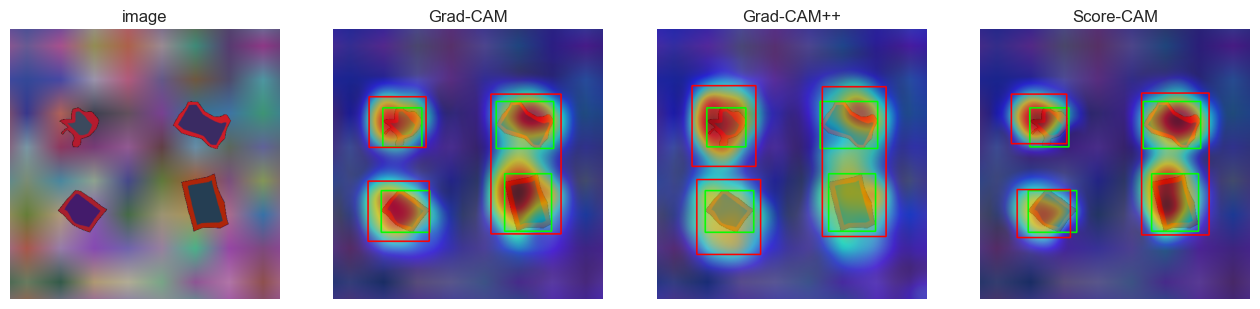
\includegraphics[width=\textwidth]{fig_vgg16_base_d4b.png}
         \caption{Explanation example from d4b dataset.}
         \label{fig:vgg16_base_explanation_d4b}
    \end{subfigure}
    \begin{subfigure}[b]{\textwidth}
         \centering
         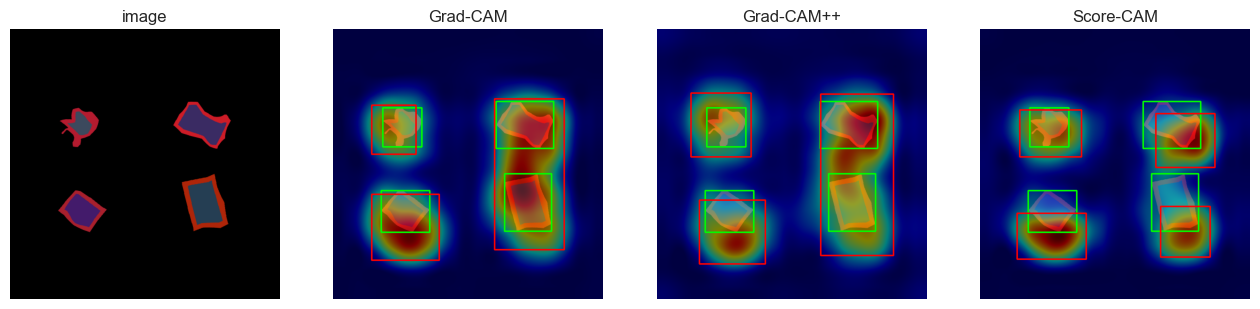
\includegraphics[width=\textwidth]{fig_vgg16_base_d4t.png}
         \caption{Explanation example from d4t dataset.}
         \label{fig:vgg16_base_explanation_d4t}
    \end{subfigure}
    \caption[Explanation maps for localization methods on VGG16 network]{Explanation maps for localization methods on VGG16 network. Heat maps show the activated image areas for the ground truth class. Annotations are given for ground truth (green) and predicted (red) bounding boxes.}
    \caption*{Source: Author}
    \label{fig:vgg16_base_explanation}
    \end{center}
\end{figure}

To prove our indication that Grad-CAM++ activates on larger areas, we measured the the number of activated pixels and the average pixel value of each score map computed using the CAM-based methods for VGG16 on the synthetic datasets. We then averaged all pixel activation counts and call this metric the average pixel activations in the score map. We also computed the average of score map average pixel values for the dataset and call this metric the average energy for the score maps. Both average pixel count and average energy enable us to compare the mean of  activated areas in the score map for the different CAM-based methods.

Figure \ref{fig:vgg16_base_pixel_energy} illustrates the average pixel activation counts and the average pixel energy in the score maps for each dataset. We clearly observe that Grad-CAM++ has the highest number of activated pixels and the highest average pixel value, backing our assumption that Grad-CAM++ activates on larger areas, which is impacting precision and recall.

Finally, we see a similar trend in pair-wise discrepancies between b-variant and t-variant datasets having the same number of object instances as observed for the VGG16-GAP network.  

\begin{figure}[h]
    \begin{center}       
    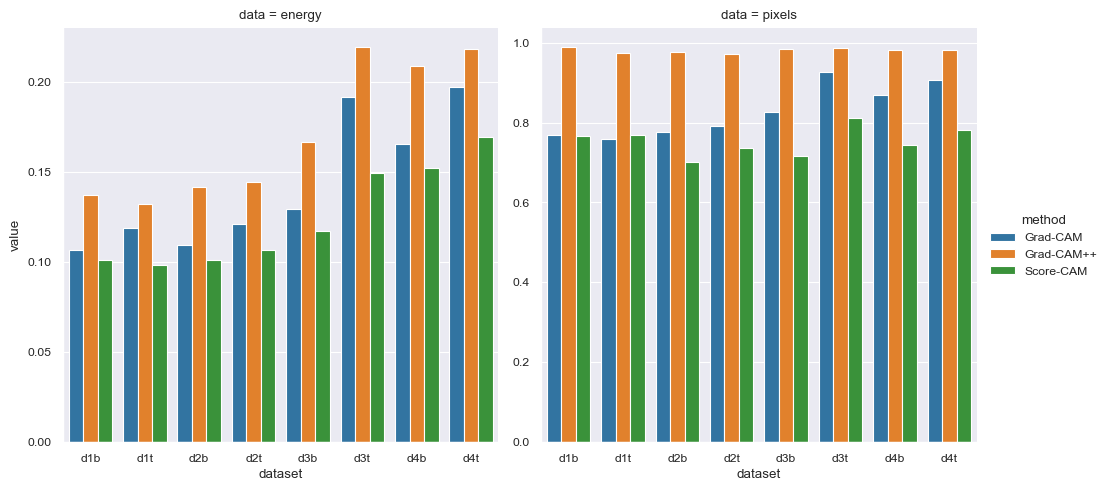
\includegraphics[width=0.95\textwidth]{fig_vgg16_base_pixel_energy.png}
    \caption[Average score map pixel activations and energy for CAM-based methods in VGG16]{Average score map pixel activations and energy for CAM-based methods in VGG16.}
    \caption*{Source: Author}
    \label{fig:vgg16_base_pixel_energy}
    \end{center}
\end{figure}

\subsubsection{ResNet-50}
Localization performance results for the ResNet-50 network on the synthetic dataset are illustrated in Table \ref{tab:maxboxaccv3_recall_resnet50_synthetic} for MaxBoxAccV3 recall, in Table \ref{tab:maxboxaccv3_precision_resnet50_synthetic} for MaxBoxAccV3 precision and in Table \ref{tab:pxap_resnet50_synthetic} for PxAP. Here Grad-CAM is not evaluated as it is identical to CAM for architectures with a \acrshort{gap} architecture.

\begin{table}[h]
\centering
\begin{tabular}{lrrrrrrrr}
\toprule
 & \multicolumn{8}{c}{ResNet-50 synthetic (MaxBoxAccV3 recall)} \\
method & d1b & d1t & d2b & d2t & d3b & d3t & d4b & d4t \\
\cmidrule(lr){1-1} \cmidrule(lr){2-9}
CAM & \color{purple} \bfseries 84.00 & \color{purple} \bfseries 74.67 & \color{purple} \bfseries 67.08 & \color{purple} \bfseries 71.08 & \color{purple} \bfseries 62.89 & \color{purple} \bfseries 62.61 & \color{purple} \bfseries 59.29 & \color{purple} \bfseries 58.71 \\
Grad-CAM++ & 85.33 & 75.67 & \color{teal} \bfseries \underline{69.33} & 72.08 & \color{teal} \bfseries \underline{66.06} & 65.00 & \color{teal} \bfseries \underline{61.79} & \color{teal} \bfseries \underline{61.13} \\
Score-CAM & \color{teal} \bfseries \underline{85.50} & \color{teal} \bfseries \underline{77.00} & 68.92 & \color{teal} \bfseries \underline{73.58} & 64.89 & \color{teal} \bfseries 65.50 & 61.63 & 60.58 \\
\cmidrule(lr){1-1} \cmidrule(lr){2-9}
MinMaxCAM & 80.33 & \color{purple} \bfseries \underline{68.17} & \color{purple} \bfseries \underline{59.17} & \color{purple} \bfseries \underline{59.08} & \color{purple} \bfseries \underline{56.50} & \color{purple} \bfseries \underline{56.11} & \color{purple} \bfseries \underline{55.92} & \color{purple} \bfseries \underline{52.87} \\
Grad-CAM++ & \color{teal} \bfseries 80.83 & 69.17 & \color{teal} \bfseries 63.83 & 61.92 & \color{teal} \bfseries 61.00 & \color{teal} \bfseries 59.94 & \color{teal} \bfseries 58.96 & \color{teal} \bfseries 57.08 \\
Score-CAM & \color{purple} \bfseries \underline{79.00} & \color{teal} \bfseries 71.17 & 61.00 & \color{teal} \bfseries 62.50 & 58.44 & 59.11 & 58.71 & 56.83 \\
\bottomrule
\end{tabular}
\caption[MaxBoxAccV3 recall for ResNet-50 on synthetic datasets]{MaxBoxAccV3 recall for ResNet-50 on synthetic datasets. First 3 rows show evaluation results for CAM-based methods evaluated on the non-regularized model. Last 3 rows show results for CAM-based models evaluated on MinMaxCAM-regularized model.  Column-wise minimum and maximum per sub-table are highlighted in red and green. Global column-wise minimum and maximum are underlined.}
\label{tab:maxboxaccv3_recall_resnet50_synthetic}
\end{table}

\begin{table}[h]
\centering
\begin{tabular}{lrrrrrrrr}
\toprule
 & \multicolumn{8}{c}{ResNet-50 synthetic (MaxBoxAccV3 precision)} \\
method & d1b & d1t & d2b & d2t & d3b & d3t & d4b & d4t \\
\cmidrule(lr){1-1} \cmidrule(lr){2-9}
CAM & \color{purple} \bfseries 75.30 & \color{purple} \bfseries 59.95 & \color{purple} \bfseries 69.48 & \color{purple} \bfseries 73.63 & \color{purple} \bfseries 68.29 & \color{purple} \bfseries 66.17 & \color{purple} \bfseries 65.83 & \color{purple} \bfseries 65.50 \\
Grad-CAM++ & 76.75 & 61.45 & \color{teal} \bfseries \underline{70.99} & 73.84 & \color{teal} \bfseries \underline{70.14} & 67.96 & 66.94 & \color{teal} \bfseries \underline{66.57} \\
Score-CAM & \color{teal} \bfseries \underline{77.58} & \color{teal} \bfseries \underline{64.77} & 69.51 & \color{teal} \bfseries \underline{74.60} & 69.25 & \color{teal} \bfseries \underline{68.70} & \color{teal} \bfseries \underline{67.75} & 65.82 \\
\cmidrule(lr){1-1} \cmidrule(lr){2-9}
MinMaxCAM & 70.21 & \color{purple} \bfseries \underline{49.82} & \color{purple} \bfseries \underline{61.23} & \color{purple} \bfseries \underline{60.03} & \color{purple} \bfseries \underline{61.27} & \color{purple} \bfseries \underline{59.88} & \color{purple} \bfseries \underline{62.59} & \color{purple} \bfseries \underline{58.82} \\
Grad-CAM++ & \color{teal} \bfseries 71.31 & 53.73 & \color{teal} \bfseries 64.93 & \color{teal} \bfseries 62.81 & \color{teal} \bfseries 63.74 & \color{teal} \bfseries 62.68 & \color{teal} \bfseries 63.85 & \color{teal} \bfseries 61.90 \\
Score-CAM & \color{purple} \bfseries \underline{68.87} & \color{teal} \bfseries 55.41 & 61.61 & 62.07 & 62.13 & 62.09 & 63.64 & 61.30 \\
\bottomrule
\end{tabular}
\caption[MaxBoxAccV3 precision for ResNet-50 on synthetic datasets]{MaxBoxAccV3 precision for ResNet-50 on synthetic datasets. First 3 rows show evaluation results for CAM-based methods evaluated on the non-regularized model. Last 3 rows show results for CAM-based models evaluated on MinMaxCAM-regularized model. Column-wise minimum and maximum per sub-table are highlighted in red and green. Global column-wise minimum and maximum are underlined.}
\label{tab:maxboxaccv3_precision_resnet50_synthetic}
\end{table}

\begin{table}[H]
\centering
\begin{tabular}{lrrrrrrrr}
\toprule
 & \multicolumn{8}{c}{ResNet-50 synthetic (PxAP)} \\
method & d1b & d1t & d2b & d2t & d3b & d3t & d4b & d4t \\
\cmidrule(lr){1-1} \cmidrule(lr){2-9} 
CAM & \color{purple} \bfseries 76.85 & \color{purple} \bfseries 65.98 & \color{purple} \bfseries 75.60 & \color{purple} \bfseries 77.27 & 75.32 & \color{purple} \bfseries 73.97 & 74.00 & \color{purple} \bfseries 71.46 \\
Grad-CAM++ & \color{teal} \bfseries 78.02 & 68.86 & \color{teal} \bfseries 76.97 & 78.03 & \color{teal} \bfseries 76.93 & 74.69 & \color{teal} \bfseries 75.31 & 72.10 \\
Score-CAM & 77.97 & \color{teal} \bfseries 69.36 & 76.09 & \color{teal} \bfseries 79.37 & \color{purple} \bfseries 74.63 & \color{teal} \bfseries 75.58 & \color{purple} \bfseries 72.83 & \color{teal} \bfseries 72.92 \\
\cmidrule(lr){1-1} \cmidrule(lr){2-9} 
MinMaxCAM & \color{purple} \bfseries 71.11 & \color{purple} \bfseries 56.26 & \color{purple} \bfseries 63.38 & \color{purple} \bfseries 66.11 & 67.64 & \color{purple} \bfseries 66.99 & \color{purple} \bfseries 68.71 & \color{purple} \bfseries 64.74 \\
Grad-CAM++ & \color{teal} \bfseries 72.56 & 59.92 & \color{teal} \bfseries 66.74 & 68.09 & \color{teal} \bfseries 70.15 & \color{teal} \bfseries 69.25 & \color{teal} \bfseries 70.83 & 66.89 \\
Score-CAM & 71.43 & \color{teal} \bfseries 61.04 & 65.57 & \color{teal} \bfseries 68.20 & \color{purple} \bfseries 67.23 & 68.20 & 69.15 & \color{teal} \bfseries 67.20 \\
\bottomrule
\end{tabular}
\caption[PxAP for ResNet-50 on synthetic datasets]{PxAP for ResNet-50 on synthetic datasets. First 3 rows show evaluation results for CAM-based methods evaluated on the non-regularized model. Last 3 rows show results for CAM-based models evaluated on MinMaxCAM-regularized model. Column-wise minimum and maximum per sub-table are highlighted in red and green. Global column-wise minimum and maximum are underlined.}
\label{tab:pxap_resnet50_synthetic}
\end{table}

A similar trend as for VGG16-GAP and VGG16 networks can be observed: Localization performance decreases for increasing number of object instances in images. 

Grad-CAM++ and Score-CAM localization methods perform better than CAM, both for the non-regularized model and for the MinMaxCAM-regularized model. Chattopadhay \textit{et al.} \cite{chattopadhyay2017grad} visually illustrated how taking a weighted combination of positive partial derivatives instead of a global average solves the problem of identifying multiple occurrences of the same class in an image and improper object localization. We quantitatively show that this statement holds for most synthetic datasets on the ResNet-50 network.

The CAM-localization (MinMaxCAM method in the tables) evaluation on the MinMaxCAM-regularized model has lower metric values than on the non-regularized model. There is room for improvement as we haven't optimized the hyper parameters for MinMaxCAM regularization during training. Still, it can be observed that Grad-CAM++ and Score-CAM both improve on the CAM localization results for the MinMaxCAM-regularized model. This means that localization trends of non-regularized model transfer to the regularized model.

\subsection{ImageNet dataset}
In this section we evaluate localization performance using CAM-based methods for the \acrshort{wsol} task on the ImageNet validation dataset. As evaluation metrics, we use the multi-instance localization metrics MaxBoxAccV3 recall and precision. In addition we report the MaxBoxAcc and MaxBoxAccV2 metrics to benchmark our trained models with results provided by Choe \textit{et al.} \cite{choe2020evaluating} where appropriate. \acrfull{pxap} cannot be used as localization metric because the ImageNet dataset has no ground truth segmentation masks. In following sections, results for VGG16-GAP and ResNet-50 architectures are discussed.

\subsubsection{VGG16-GAP}
We modified a pretrained VGG16 network into the VGG16-GAP network by replacing the dense network layers of VGG16 with a \acrshort{gap} layer followed by a single fully connected layer. This newly constructed network is fine-tuned until the loss of the validation dataset hasn't decreased for five consecutive training epochs. The localization results of VGG16-GAP on the ImageNet validation dataset are illustrated in Table \ref{tab:metrics_vgg16_gap_imagenet}.

\begin{table}[h]
\centering
\begin{tabular}{lrrrr}
\toprule
 & & & \multicolumn{2}{c}{MaxBoxAccV3} \\
method & MaxBoxAcc & MaxBoxAccV2 & precision & recall \\
\cmidrule(lr){1-1} \cmidrule(lr){2-5}
CAM & 61.19 & 60.22 & \color{purple} \bfseries 36.73 & 38.44 \\
Grad-CAM++ & \color{teal} \bfseries 61.29 & \color{teal} \bfseries 60.43 & 36.87 & \color{teal} \bfseries 38.66 \\
Score-CAM & \color{purple} \bfseries 58.44 & \color{purple} \bfseries 57.56 & \color{teal} \bfseries 37.33 & \color{purple} \bfseries 36.48 \\
\bottomrule
\end{tabular}
\caption[Localization metrics for VGG16-GAP on ImageNet]{Localization metrics for VGG16-GAP on ImageNet. Column-wise minimum and maximum are highlighted in red and green.}
\label{tab:metrics_vgg16_gap_imagenet}
\end{table}

The values for the metrics MaxBoxAcc ($61.19$) and MaxBoxAccV2 ($60.22$) for the \acrshort{cam} method closely match the results reported by Choe \textit{et al.} \cite{choe2020evaluating}. Our VGG16-GAP model is thus able to reproduce the results in the \acrshort{wsol} evaluation paper.

The MaxBoxAccV3 precision and recall values for VGG16-GAP on the ImageNet dataset are much lower than the values for the synthetic dataset. This is to be expected as the ImageNet dataset is far more complex: It has 1000 different classes and a training dataset of 1.2 million images, where the synthetic datasets have only 9 different classes with a training dataset of 1000 images. The model trained on the ImageNet dataset has a classification accuracy of 67.1\%, where classification accuracy for models trained on the synthetic datasets is close to 100\%. 

MaxBoxAccV3 recall for Score-CAM is about 2 percentage points lower than CAM and Grad-CAM++. Intuitively, Score-CAM could be impacted more than the other CAM-based methods by the relatively low classification accuracy for the ImageNet dataset, as Score-CAM computes the score map based on the impact of feature maps on the predicted score. Figure \ref{fig:explain_vgg16_gap_imagenet} shows for two images the areas activated in the score map for each evaluated CAM-based method. We can observe that Grad-CAM++ highlights a larger area of the object of interest, resulting in a larger predicted (red) bounding box that has a smaller \acrshort{iou} with the ground truth (green) bounding box, and thus impacting the MaxBoxAccV3 recall. 

\begin{figure}[h]
\begin{center}
    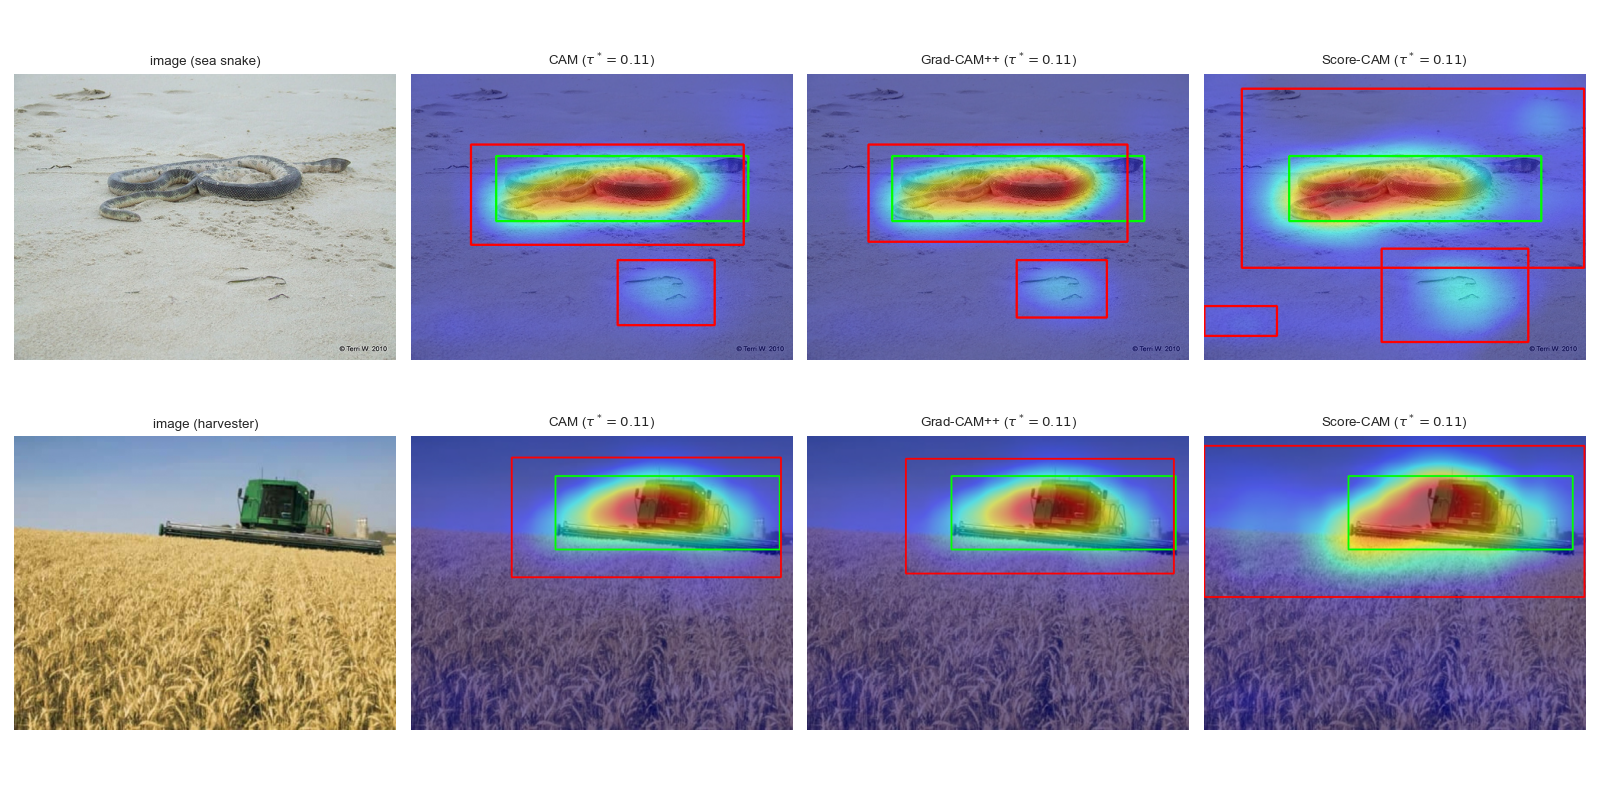
\includegraphics[width=\textwidth]{fig_explain_vgg16_gap_imagenet.png}
    \caption[Explanation maps of CAM-based localization for VGG16-GAP on ImageNet images]{Explanation maps of CAM-based localization for VGG16-GAP on ImageNet images
. Heat maps show the activated image areas for the ground truth class. Annotations are given for ground truth (green) and predicted (red) bounding boxes.}
    \caption*{Source: Author}
    \label{fig:explain_vgg16_gap_imagenet}
\end{center}
\end{figure}

The multi-instance localization metrics are determined predominantly by single-instance images in the ImageNet validation dataset as they represent the majority of images (Figure \ref{fig:imagenet_instance_distribution}). Therefore, it is interesting to split up the ImageNet validation dataset according to the number of object instances in images to evaluate localization performance in function of the number of object instances. We have evaluated these separate ImageNet datasets for the ResNet-50 network (section \ref{sec:exp_resnet50_imagenet}).

Due to time constraints, we were unable to train a MinMaxCAM-regularized model for the VGG16-GAP network on ImageNet.

\subsubsection{ResNet-50} \label{sec:exp_resnet50_imagenet}

For the ResNet-50 network we evaluate localization using CAM, Grad-CAM++ and Score-CAM on the ImageNet validation dataset, both on a model trained without regularization, and on a model trained with MinMaxCAM regularization. The results of these experiments are illustrated in Table \ref{tab:metrics_resnet50_imagenet}, where the method denoted as MinMaxCAM represents localization using the CAM method on tje MinMaxCAM-regularized model. 

\begin{table}[h]
\centering
\begin{tabular}{lrrrr}
\toprule
 & & & \multicolumn{2}{c}{MaxBoxAccV3} \\
method & MaxBoxAcc & MaxBoxAccV2 & precision & recall \\
\cmidrule(lr){1-1} \cmidrule(lr){2-5}
CAM & 57.60 & 57.25 & 30.55 & 36.58 \\
Grad-CAM++ & \color{teal} \bfseries 59.40 & \color{teal} \bfseries 58.55 & \color{teal} \bfseries 31.17 & \color{teal} \bfseries \underline{37.53} \\
Score-CAM & \color{purple} \bfseries \underline{56.19} & \color{purple} \bfseries \underline{56.35} & \color{purple} \bfseries \underline{29.60} & \color{purple} \bfseries \underline{35.92} \\
\cmidrule(lr){1-1} \cmidrule(lr){2-5}
MinMaxCAM & \color{purple} \bfseries 58.81 & \color{purple} \bfseries 57.26 & \color{teal} \bfseries \underline{43.70} & \color{purple} \bfseries 36.02 \\
Grad-CAM++ & \color{teal} \bfseries \underline{60.87} & \color{teal} \bfseries \underline{58.92} & 41.81 & \color{teal} \bfseries 37.12 \\
Score-CAM & 60.00 & 58.10 & \color{purple} \bfseries 38.70 & 36.53 \\
\bottomrule
\end{tabular}
\caption[Localization metrics for ResNet-50 on ImageNet]{Localization metrics for ResNet-50 on ImageNet. First 3 rows show evaluation results for CAM-based methods evaluated on the non-regularized model. Last 3 rows show results for CAM-based models evaluated on MinMaxCAM-regularized model. Column-wise minimum and maximum per sub-table are highlighted in red and green. Global column-wise minimum and maximum are underlined.}
\label{tab:metrics_resnet50_imagenet}
\end{table}

The MaxBoxAcc and MaxBoxAccV2 metrics for the CAM method evaluated on the non-regularized model have lower values than those reported by Choe \textit{et al.} \cite{choe2020evaluating} (57.60 and 57.25 versus 64.2 and 63.7). An explanation for this discrepancy, most likely is that we used a pretrained ResNet-50 model where the authors of the mentioned paper did a grid search on hyper parameters to improve localization. 

The MaxBoxAccV3 metric has slightly lower values than the ones we reported for the VGG16-GAP network, but the same trend can be observed: The highest recall is obtained by the Grad-CAM++ method and the Score-CAM recall is about two percentage points below Grad-CAM++'s value. 

The MaxBoxAccV3 recall difference between non-regularized and regularized models for a specific CAM-based method, is rather limited. However, MaxBoxAccV3 precision has improved substantially for the CAM-based methods evaluated on the regularized model, indicating that localization methods using this model produce fewer false positives.

MaxBoxAcc and MaxBoxAccV2 values are slightly higher for the MinMaxCAM-regularized model than for the non-regularized model. This is in contrast with the results reported by Wang \textit{et al.} \cite{wang2021minmaxcam}, who illustrated that MinMaxCAM improves MaxBoxAcc by 2.5 percentage points compared to CAM. We were unable to reproduce the results reported by the authors of the MinMaxCAM paper \cite{wang2021minmaxcam} due to unavailability of reference values for the regularization weights.

In chapter \ref{ch:methodology}, we reported the distribution of object instances over the images in the ImageNet validation dataset (Figure \ref{fig:imagenet_instance_distribution}). Because the vast majority of images in the dataset have only one object instance, the localization results may be biased towards those images. Therefore, we have split the ImageNet validation dataset into different datasets, so that each dataset has only images with fixed number of object instances. We then evaluated the CAM localization method separately on each of these datasets. The MaxBoxAccV3 recall results for these experiments are shown in Figure \ref{fig:resnet50_imagenet_inst_recall}. 

\begin{figure}[h]
    \begin{center}       
    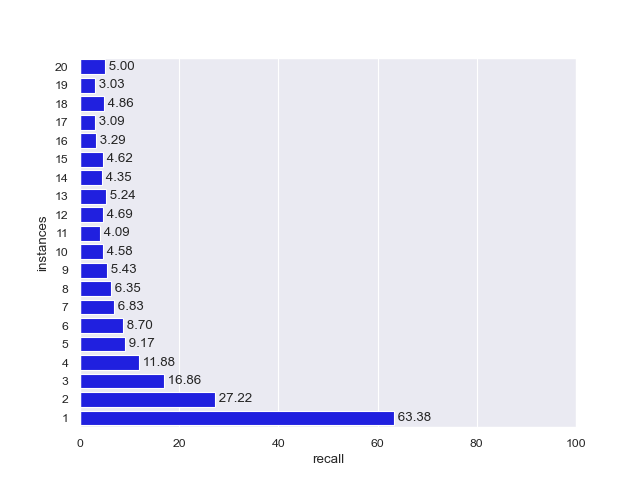
\includegraphics[width=0.8\textwidth]{fig_resnet50_imagenet_inst_recall.png}
    \caption[CAM MaxBoxAccV3 recall on ResNet-50 for ImageNet split across number object instances]{CAM MaxBoxAccV3 recall on ResNet-50 for ImageNet split across number object instances.}
    \caption*{Source: Author}
    \label{fig:resnet50_imagenet_inst_recall}
    \end{center}
\end{figure}

We observe that recall performance depends on the number of object instances in the images. Recall is highest for the single-instance dataset, and significantly drops significantly as more object instances are present in the images of a dataset. For ImageNet datasets with eight or more instances, recall seems to be rather similar. We observed a similar pattern for the synthetic datasets: Recall decreases for datasets increasing number of object instances in images.

The ImageNet dataset with single-instance images has a MaxBoxAccV3 recall of 63.38, which is close to the MaxBoxAccV2 value of 57.25 in Table \ref{tab:metrics_resnet50_imagenet}. It can be shown that for single-instance datasets, MaxBoxAccV2 and MaxBoxAccV3 are identical, as in this case, the number of images equals the number ground-truth bounding boxes, and from equations \ref{eq:boxacc}, \ref{eq:maxboxaccv2}, \ref{eq:boxaccv2} and \ref{eq:maxboxaccv3}, we can derive that MaxBoxAccV2 equals MaxBoxAccV3. The difference in the results is because the MaxBoxAccV2 value from Table \ref{tab:metrics_resnet50_imagenet} was measured on the complete ImageNet validation dataset, including images with more than one object instance.

Figure \ref{fig:resnet50_imagenet_inst_precision} illustrates MaxBoxAccV3 precision for the ImageNet datasets split by number of object instances.

\begin{figure}[h]
    \begin{center}       
    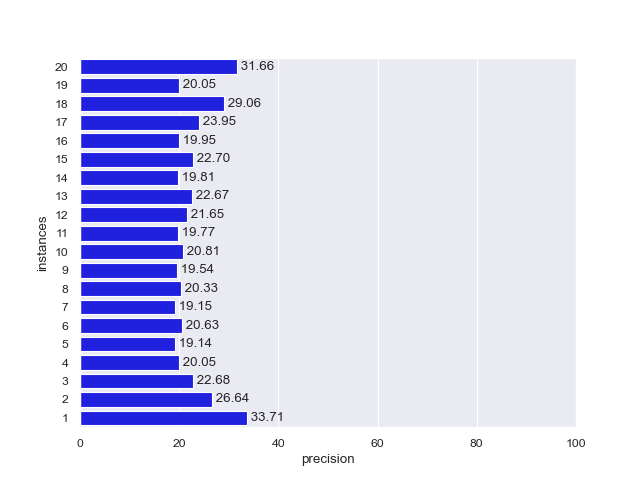
\includegraphics[width=0.8\textwidth]{fig_resnet50_imagenet_inst_precision.png}
    \caption[CAM MaxBoxAccV3 precision on ResNet-50 for ImageNet split across number object instances]{CAM MaxBoxAccV3 precision on ResNet-50 for ImageNet split across number object instances.}
    \caption*{Source: Author}
    \label{fig:resnet50_imagenet_inst_precision}
    \end{center}
\end{figure}

For  the first four datasets (instances 1 till 4), we see a drop in precision as more instances are present in images. When dataset images have more object instances, precision values don't seem to correlate with the number of instances. That means that the localization method is not generating relatively more false positives as are more object instances are present in the images. Intuitively, the more object instances in an image, the closer they are, and the higher the probability that the localization method will localize groups of instances as a single instance, which will impact recall but not precision. 
 
\section{Computational complexity}
In this section we evaluate the computational complexity of localization methods CAM, Grad-CAM++ and Score-CAM. MinMaxCAM and Grad-CAM are not measured as MinMaxCAM uses the same localization method as CAM and Grad-CAM has the same order of complexity as Grad-CAM++ due to the equal number of forward and backward passes (see Table \ref{tab:complexity_theoretical}). We measure the localization method runtime for ResNet-50 network on the 50000 images of the ImageNet validation dataset. 

The runtime of the localization methods is measured as the time it takes to compute the score map of the images. For efficiency reasons, we process batches of images for score map computation, thus the runtime measurements are also performed on batches of images. Mean and standard deviation for runtime are then computed over all batches of the dataset. Total runtime is the sum of the runtime of all batches. For runtime computation, we exclude operations that load and preprocess the images.

The results for each method are illustrated in Table \ref{tab:runtime_resnet50_imagenet}. The batch size is listed per method as it should be taken into consideration when interpreting the mean and standard deviation values.

\begin{table}[h]
\centering
\begin{tabular}{lrrrr}
\toprule
\multicolumn{2}{c}{} & \multicolumn{3}{c}{runtime (ms)} \\
method & batch size (images) & sum & mean & std \\
\cmidrule(lr){1-2} \cmidrule(lr){3-5}
CAM & 512 & 309209 & 3155 & 225 \\
Grad-CAM++ & 128 & 804349 & 2057 & 140 \\
MinMaxCAM & 512 & 299392 & 3055 & 982 \\
Score-CAM & 512 & \color{teal} \bfseries 97763413 & \color{teal} \bfseries 997585 & \color{teal} \bfseries 34463\\
\bottomrule
\end{tabular}
\caption[Method runtime for ResNet-50 on ImageNet validation dataset]{Method runtime for ResNet-50 on ImageNet validation dataset.  Column-wise maximum is highlighted in bold green.}
\label{tab:runtime_resnet50_imagenet}
\end{table}

We observe that Grad-CAM++ takes nearly three times the runtime of the CAM method. The major difference is that Grad-CAM++ requires a backward pass after each forward pass to compute gradients. This indicates that backward passes are computationally more costly than forward passes.

Each method computes a score map as a weighted combination of feature maps in the final convolutional layer. CAM computes as weights the target class related parameters learned in the single fully connected layer, which is a very cheap operation. Grad-CAM and Grad-CAM++ compute weights from feature map activations and the back-propagated gradients in the final convolutional layer.

The most computationally costly method by far is Score-CAM. This method computes the weights for the feature maps by feeding the network with the product of feature map activations with the original image to obtain the classification scores after softmax. Those scores are then used as weights to compute the score map. As ResNet-50 has 2048 channels in its final convolutional layer, this is an expensive operation.

\section{Localization improvements} \label{sec:exp_loc_improvements}

Using the iterative localization method proposed in section \ref{sec:method_localization_improvement}, we analyze the effect of this method on the ResNet-50 architecture for the synthetic and ImageNet datasets. We use the same models that were trained for the non-iterative approach.

\subsection{Recall versus precision}
The aim of the iterative approach is to improve the accurate localization of ground truth object instances. This localization accuracy is measured by the MaxBoxAccV3 recall metric. A naive approach to improving recall would be to use a localization method that exhaustively generates bounding boxes of different granularity at various locations. Such a method would accurately localize most object instances and thus have a high recall value. At the same time this method would suffer from a lot of false positives, i.e., many of the predicted object localization instances would not match with the actual ground truth localization annotations. Hence, precision would be very low. To measure the impact of the iterative localization method, we want to measure both precision and recall. Ideally, we would like to have a localization method that has good precision and recall.

\subsection{Evaluation approach}
In our iterative localization approach, we apply different mask strategies, bounding box merge strategies and iteration stop criteria in our experiments. The different parameters and their possible values are illustrated in Table \ref{tab:iterative_localizaton_parameters}.

\begin{table}[ht]
\centering
\begin{tabular}{ll}
\toprule
Parameter & Values\\
\cmidrule(lr){1-2}
Localization method & CAM, Grad-CAM++, Score-CAM, MinMaxCAM \\
Mask strategy & zero, mean, random \\
Merge strategy & add, drop, unify \\
Classification score drop threshold & 0.25, 0.5, 1.0 \\
\bottomrule
\end{tabular}
\caption[Parameters for the iterative localization approach]{Parameters for the iterative localization approach.}
\label{tab:iterative_localizaton_parameters}
\end{table}

 Due to the number of possible parameter combinations, we have to compare a lot of results. It is rather difficult to represent these results in a single table and draw conclusions from it. Therefore we graphically represent and interpret the results as follows:
\begin{itemize}
    \item Per dataset, network and localization method, we create a two-dimensional plot with recall on the horizontal axis and precision on the vertical axis. In this plot, for each of the different combinations of mask strategies, merge strategies and stop criteria, an experiment is run and its resulting precision and recall are added to the plot.
    \item The precision and recall for the non-iterative approach is plotted as two orthogonal lines: A horizontal line for precision and vertical line for recall. We use the precision and recall from the non-iterative approach as baseline to compare with results from the iterative approach.
    \item The horizontal and vertical lines of the baseline create four quadrants which allow easy graphical interpretation of iterative localization results depending in which quadrant a result is situated.
    \begin{itemize}
        \item Bottom left: Worse precision and recall than the baseline.
        \item Top left: Better precision but worse recall than baseline.
        \item Bottom right: Better recall but worse precision than baseline.
        \item Top right: Better precision and recall than the baseline.
    \end{itemize}
\end{itemize}

\subsection{Evaluation for ResNet-50 on synthetic datasets} \label{sec:exp_iter_resnet50_syn}
Here we evaluate the results of the iterative localization for the ResNet-50 network on the synthetic test datasets. We only evaluate datasets that have images with a background to analyze the effect of using different bounding box mask strategies. The localization methods used are CAM, Grad-CAM++, Score-CAM and MinMaxCAM. The former three methods are evaluated on a model trained without regularization while the latter is evaluated on a model trained with MinMaxCAM regularization. 

We will evaluate iterative localization done both with oracle based masks and score map based masks, to compare the impact of using both mask techniques on multiple-instance localization performance.

\subsubsection{Oracle-based iterative localization}

As explained in section \ref{sec:method_localization_improvement}, we use the \acrshort{gt}-based bounding boxes mask method as an oracle, i.e. for providing upper bounds on the performance that could be obtained when iterative localization would be guided by the ground truth. Figure \ref{fig:prec_iter_resnet50_syn_d1b} illustrates localization results for the d1b dataset.

\begin{figure}[h]
    \begin{center}       
    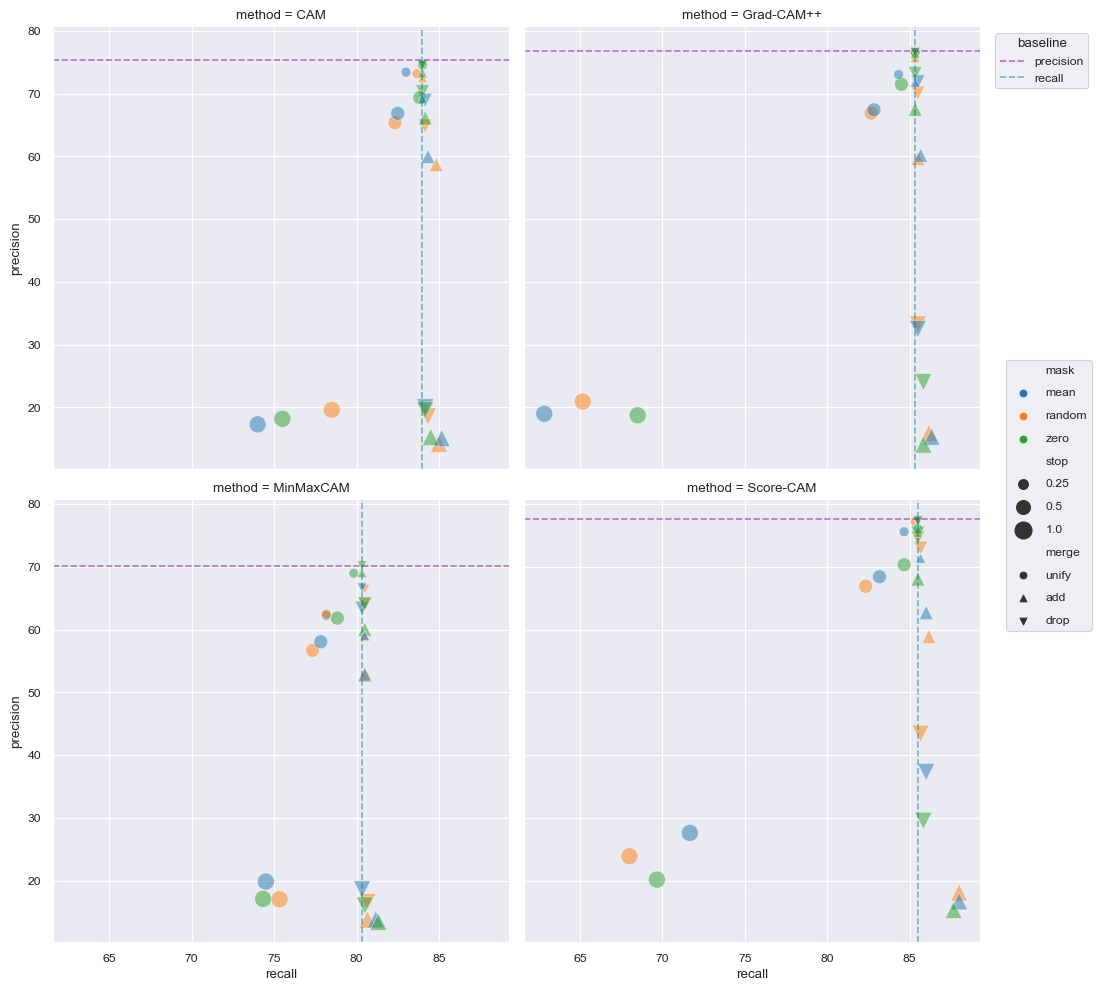
\includegraphics[width=0.99\textwidth]{images/fig_iter_resnet50_syn_d1b.png}
    \caption[Oracle-based iterative localization performance for ResNet-50 on synthetic dataset d1b]{Oracle-based iterative localization performance for ResNet-50 on synthetic dataset d1b. The cross-hair lines mark the best precision and recall for non-iterative localization.}
    \caption*{Source: Author}
    \label{fig:prec_iter_resnet50_syn_d1b}
    \end{center}
\end{figure}

When comparing with the baseline, we observe that for all methods, recall can be improved by using the 'add' merge strategy and classification score drop threshold 1.0. This threshold actually means that no iteration stop criterion is used. It's easy to see that this threshold has the worst precision for any mask or merge strategy. The 'add' merge strategy improves recall but at the cost of decreased precision, as this strategy causes more false positives. The relatively small gain in recall is to be expected for a dataset with single-instance object images where the baseline already has a high localization performance.

\begin{figure}[h]
    \begin{center}       
    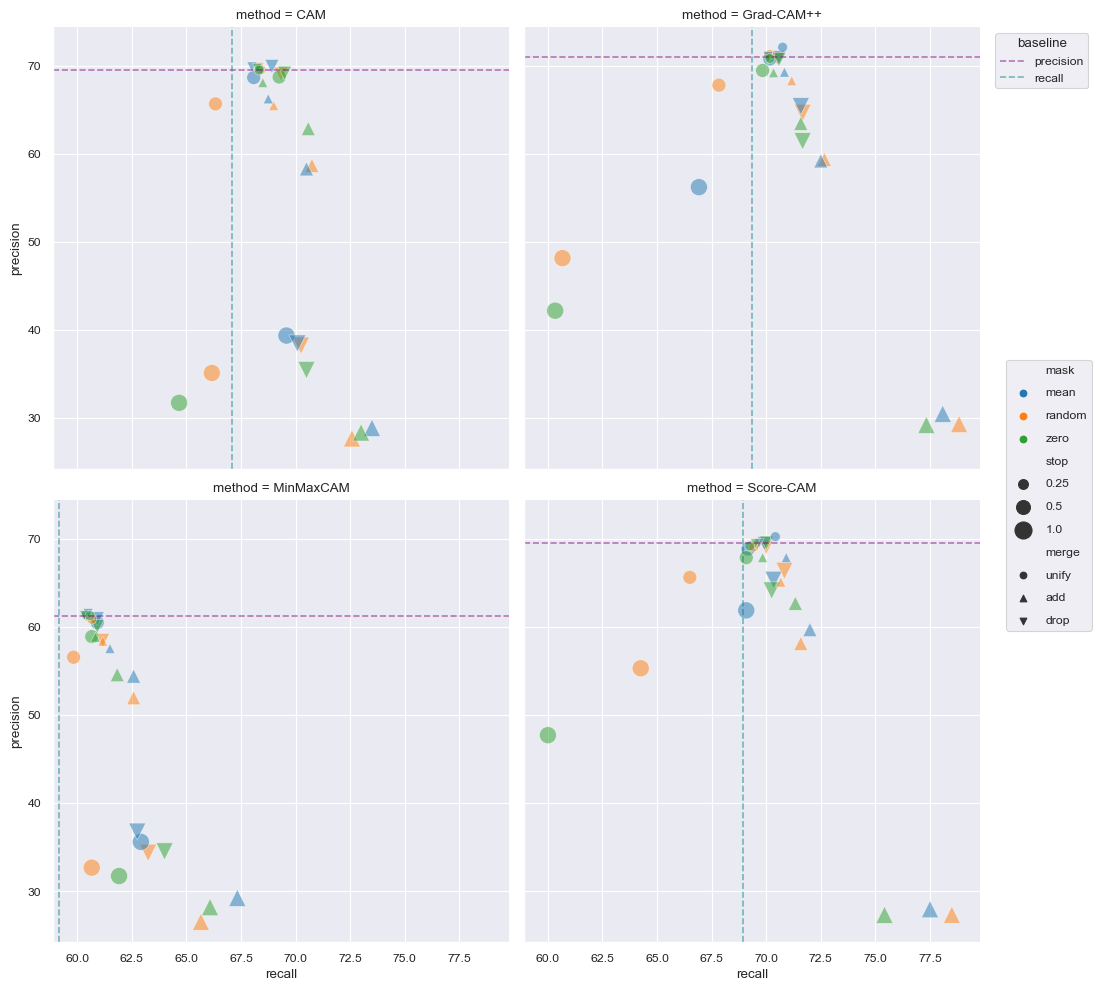
\includegraphics[width=0.99\textwidth]{images/fig_iter_resnet50_syn_d2b.png}
    \caption[Oracle-based iterative localization performance for ResNet-50 on synthetic dataset d2b]{Oracle-based iterative localization performance for ResNet-50 on synthetic dataset d2b. The cross-hair lines mark the best precision and recall for non-iterative localization.}
    \caption*{Source: Author}
    \label{fig:prec_iter_resnet50_syn_d2b}
    \end{center}
\end{figure}

Iterative localization results for the d2b dataset are shown in Figure \ref{fig:prec_iter_resnet50_syn_d2b}. Looking at the upper right quadrant, we can observe that there are iterative approaches that improve both precision and recall for all localization methods except MinMaxCAM. For Grad-CAM++ and Score-CAM, applying the 'unify' merge strategy, combined with 'mean' mask strategy and stop criterion with classification drop threshold of 0.25, provides the best precision and recall improvements compared to the baseline. For CAM, applying the 'drop' merge strategy is the best approach. For MinMaxCAM, any iteration strategy improve recall at the cost of lower precision. 

The highest recall improvement at the cost of precision, is provided by the 'add' merge strategy combined with iteration drop criterion 1.0. The worst precision and recall results are observed for the 'unify' merge strategy with drop criterion 1.0. Intuitively, masking images with bounding boxes found in previous iterations, and unifying newly predicted bounding boxes with overlapping boxes of previous iterations, increases the probability of no longer matching predicted bounding boxes with ground truth boxes, and thus impacting recall.

\begin{figure}[h]
    \begin{center}       
    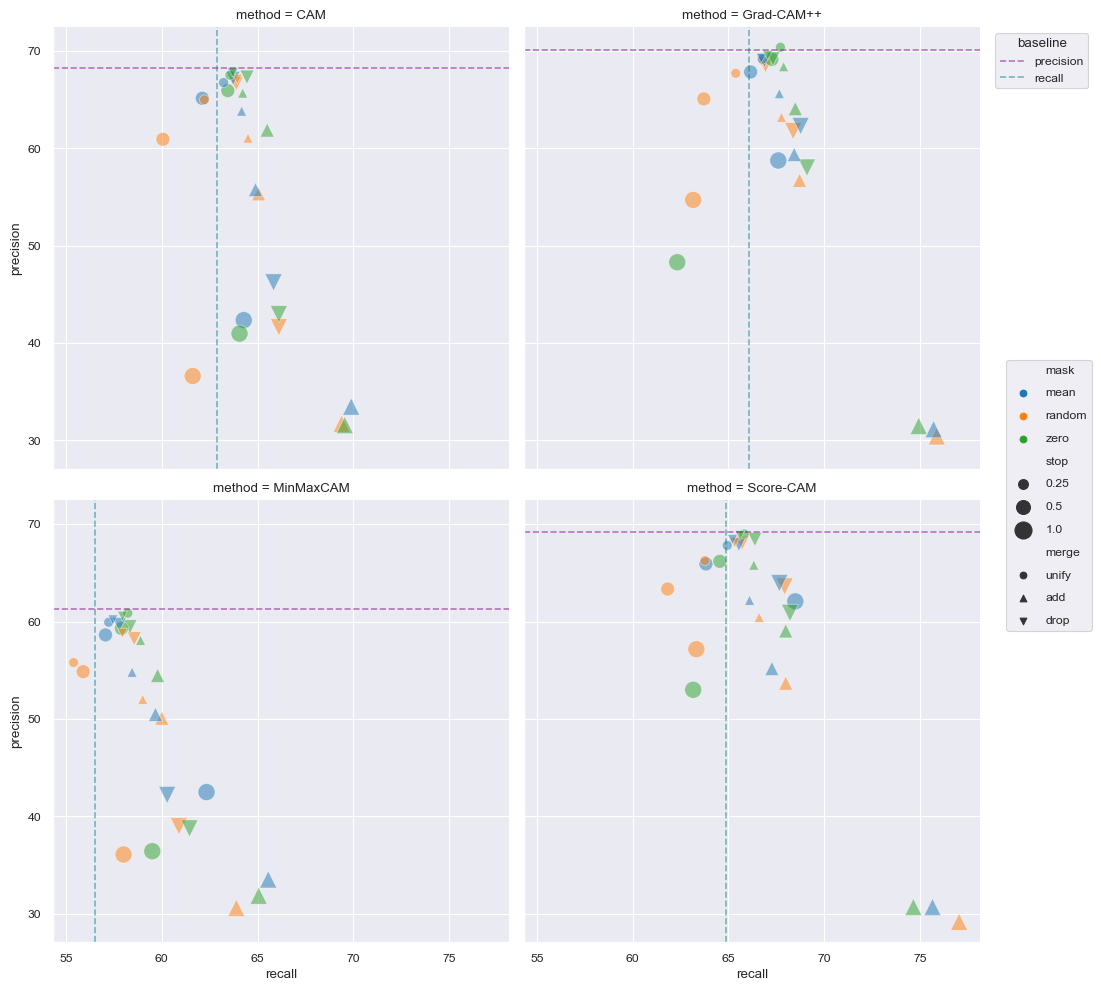
\includegraphics[width=0.99\textwidth]{images/fig_iter_resnet50_syn_d3b.png}
    \caption[Oracle-based iterative localization performance for ResNet-50 on synthetic dataset d3b]{Oracle-based iterative localization performance for ResNet-50 on synthetic dataset d3b. The cross-hair lines mark the best precision and recall for non-iterative localization.}
    \caption*{Source: Author}
    \label{fig:prec_iter_resnet50_syn_d3b}
    \end{center}
\end{figure}

Figure \ref{fig:prec_iter_resnet50_syn_d3b} illustrates the iterative localization results for the d3b dataset. We observe that the iterative approach can improve recall at the cost of precision for all localization methods. Applying the 'add' merge strategy and stop criterion threshold of 1.0 gives the highest recall gain, but at the cost of high precision loss. For Grad-CAM++, both precision and recall can be improved using the 'unify' merge and 'zero' mask strategy, combined with iteration stop criterion 0.25.

The iterative localization metrics for the d4b dataset are shown in Figure \ref{fig:prec_iter_resnet50_syn_d4b}. As for the d3b dataset, recall can be improved at the cost of precision for all localization methods. The 'add' merge strategy with stop threshold 1.0 provides the highest gain in recall at the cost of substantially decreasing precision.

\begin{figure}[h]
    \begin{center}       
    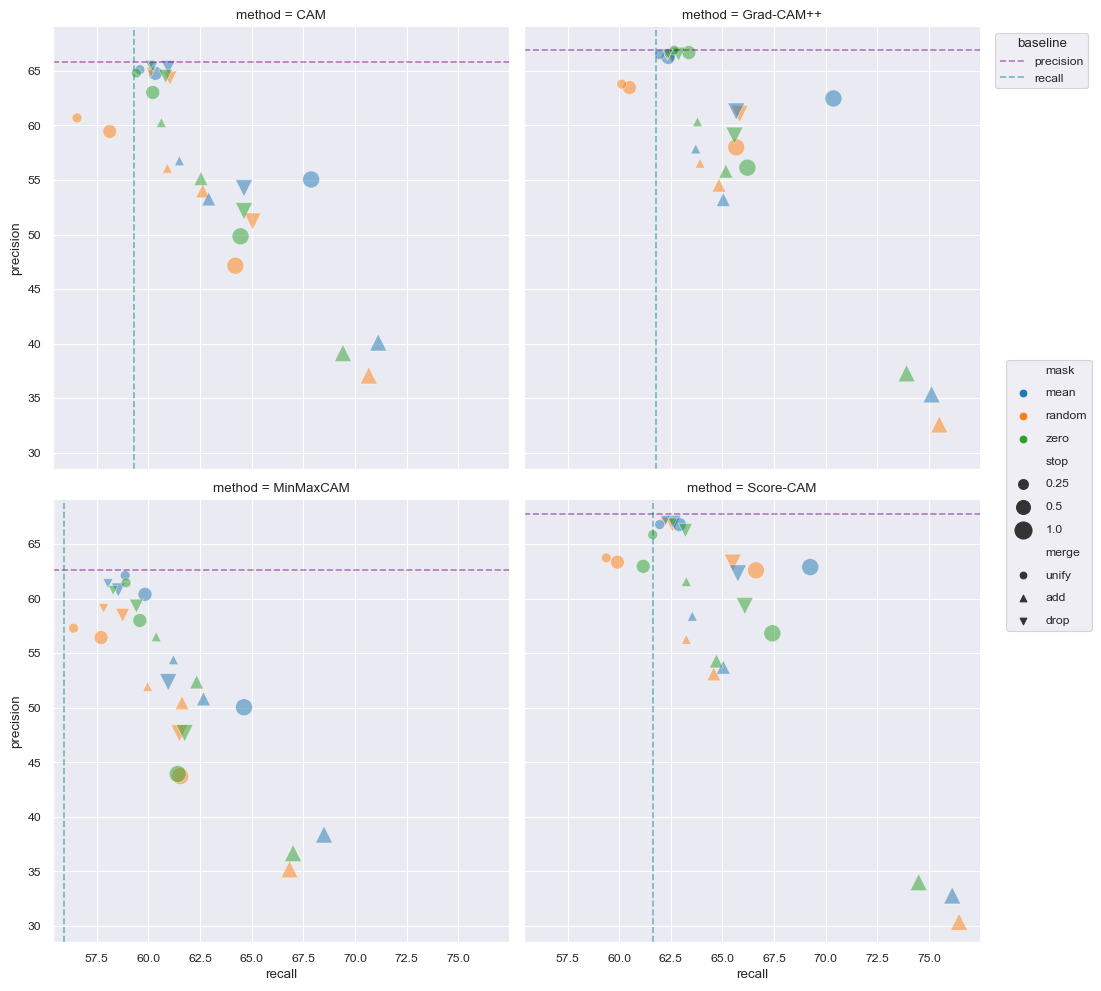
\includegraphics[width=0.99\textwidth]{images/fig_iter_resnet50_syn_d4b.png}
    \caption[Oracle-based iterative localization performance for ResNet-50 on synthetic dataset d4b]{Oracle-based iterative localization performance for ResNet-50 on synthetic dataset d4b. The cross-hair lines mark the best precision and recall for non-iterative localization.}
    \caption*{Source: Author}
    \label{fig:prec_iter_resnet50_syn_d4b}
    \end{center}
\end{figure}

\subsubsection{Score map based iterative localization}

As the score map based mask technique doesn't depend on ground truth information, we can effectively evaluate multiple-instance localization performance for the \acrshort{wsol} task. We do this for the same CAM-based methods, networks and datasets as done for the experiments using GT-based bounding box masking technique. Figure \ref{fig:prec_iter_mask_cam_resnet50_syn_d1b} illustrates score map based localization results for the d1b dataset.

\begin{figure}[h]
    \begin{center}       
    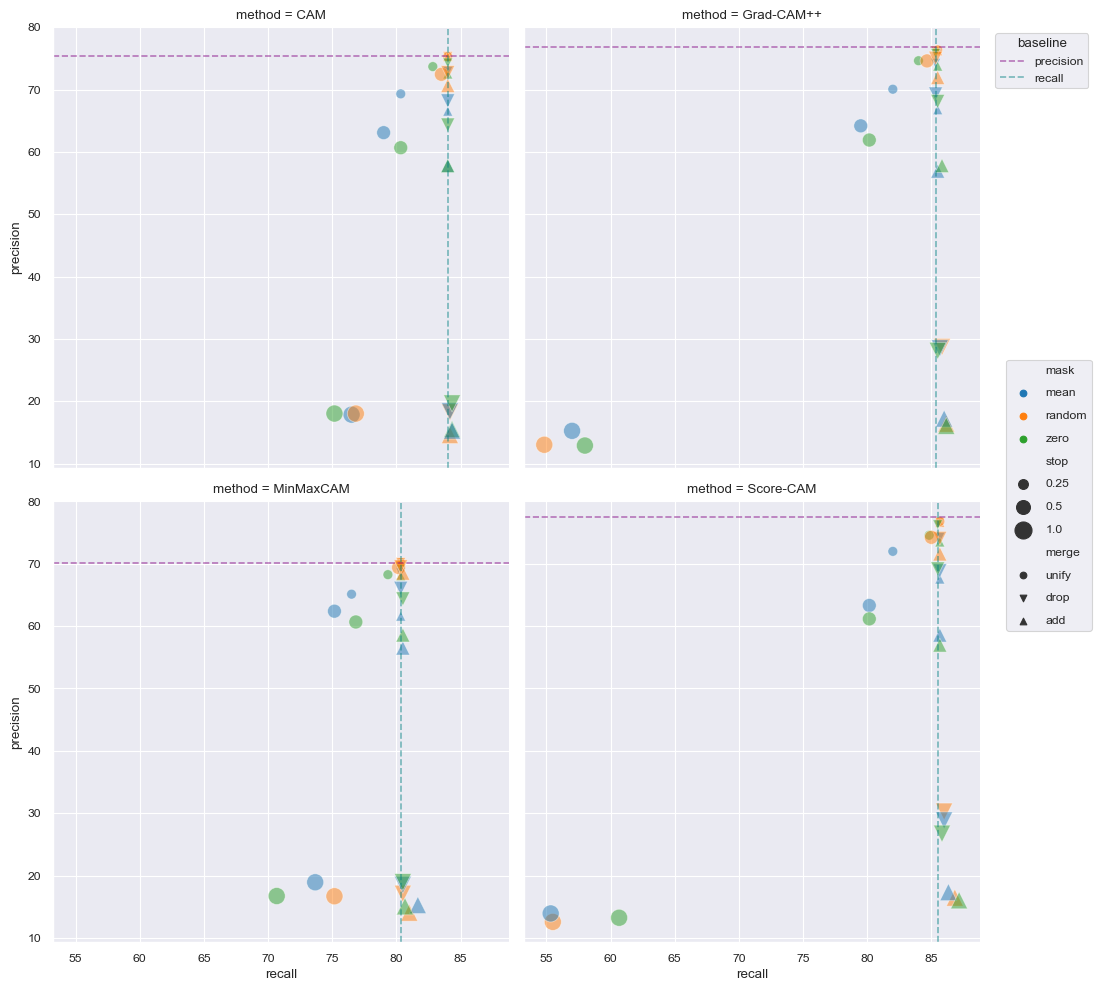
\includegraphics[width=0.99\textwidth]{fig_iter_mask_cam_resnet50_syn_d1b.png}
    \caption[Score map based iterative localization performance for ResNet-50 on synthetic dataset d1b]{Score map based iterative localization performance for ResNet-50 on synthetic dataset d1b. The cross-hair lines mark the best precision and recall for non-iterative localization.}
    \caption*{Source: Author}
    \label{fig:prec_iter_mask_cam_resnet50_syn_d1b}
    \end{center}
\end{figure}

We can observe a similar trend when compared to oracle-based iterative localization: For all methods, recall can be improved by using the 'add' merge strategy and classification score drop threshold 1.0. The 'add' merge strategy improves recall but at the cost of decreased precision. However, the recall improvements are smaller for score map iterative localization. Intuitively, the rather coarse score map threshold used to compute the score map based mask may yield localization information that is less accurate than the oracle based mask that is based on ground truth information.

Iterative localization results for the d2b dataset are shown in Figure \ref{fig:prec_iter_mask_cam_resnet50_syn_d2b}. Where both localization precision and recall could be improved in oracle-based iterative localization, we don't see the same trend for score map based iterative localization. The 'add' merge strategy with iteration drop criterion 1.0 provides the highest recall improvements, albeit marginal, at the cost of decreased precision.

\begin{figure}[h]
    \begin{center}       
    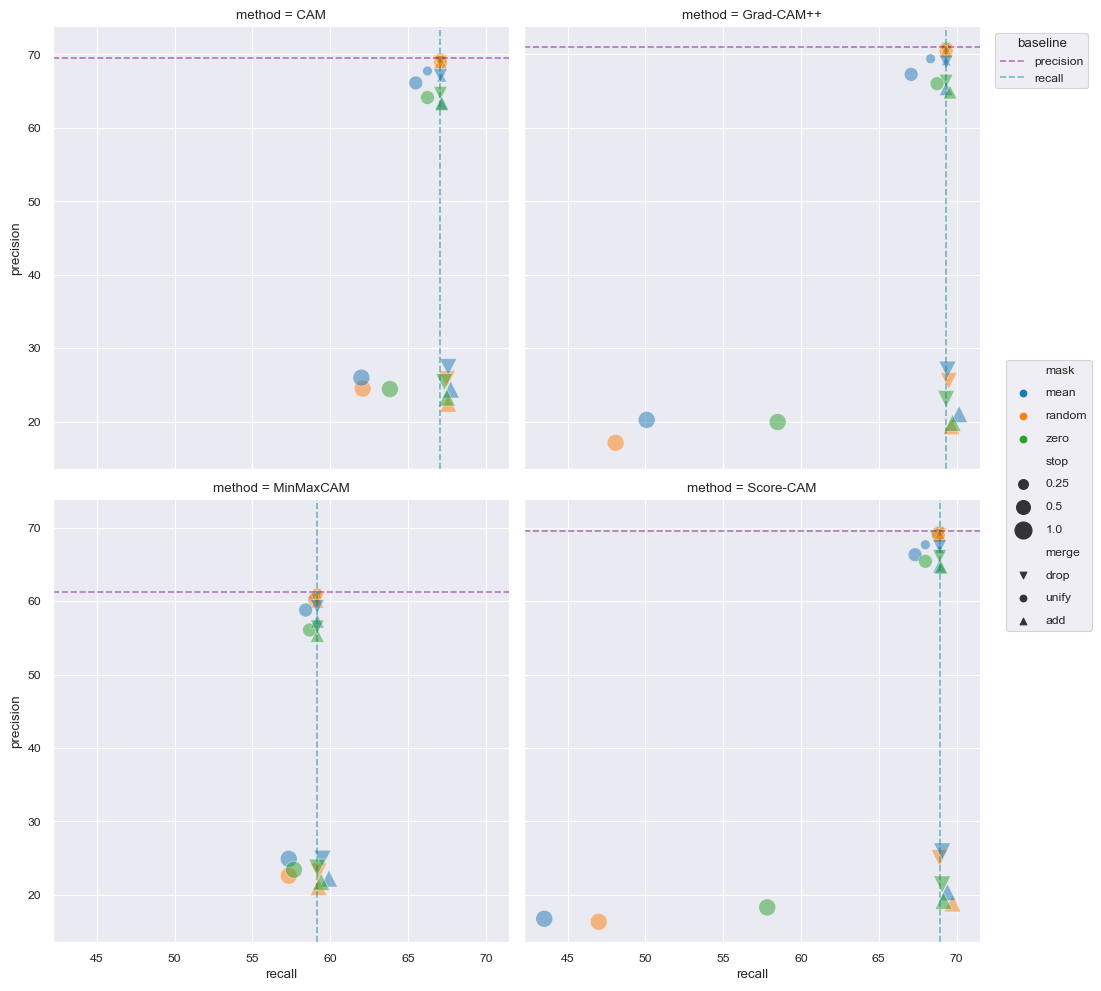
\includegraphics[width=0.99\textwidth]{fig_iter_mask_cam_resnet50_syn_d2b.png}
    \caption[Score map based iterative localization performance for ResNet-50 on synthetic dataset d2b]{Score map based iterative localization performance for ResNet-50 on synthetic dataset d2b. The cross-hair lines mark the best precision and recall for non-iterative localization.}
    \caption*{Source: Author}
    \label{fig:prec_iter_mask_cam_resnet50_syn_d2b}
    \end{center}
\end{figure}

Figure \ref{fig:prec_iter_mask_cam_resnet50_syn_d3b} illustrates the iterative localization results for the d3b dataset. We observe that the iterative approach can improve recall at the cost of precision for all localization methods. Applying the 'add' merge strategy and stop criterion threshold of 1.0 gives the highest recall gain, but at the cost of high precision loss. Grad-CAM++ and Score-CAM provide the highest recall for the 'add' merge strategy. This is similar to what we observed for oracle-based iterative localization, albeit that the recall gain for score map based iterative localization is much smaller.

\begin{figure}[h]
    \begin{center}       
    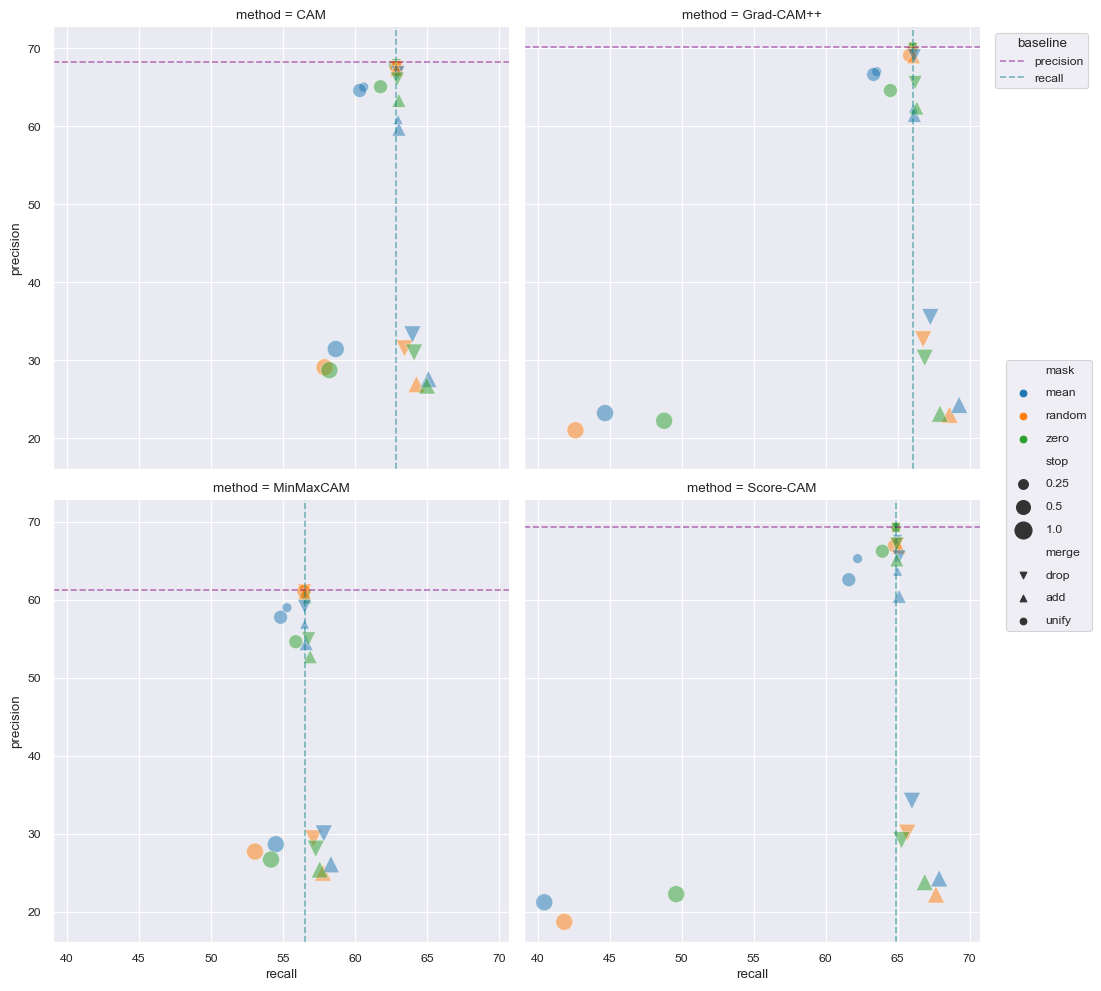
\includegraphics[width=0.99\textwidth]{fig_iter_mask_cam_resnet50_syn_d3b.png}
    \caption[Score map based iterative localization performance for ResNet-50 on synthetic dataset d3b]{Score map based iterative localization performance for ResNet-50 on synthetic dataset d3b. The cross-hair lines mark the best precision and recall for non-iterative localization.}
    \caption*{Source: Author}
    \label{fig:prec_iter_mask_cam_resnet50_syn_d3b}
    \end{center}
\end{figure}

The iterative localization metrics for the d4b dataset are shown in Figure \ref{fig:prec_iter_mask_cam_resnet50_syn_d4b}. As for the d3b dataset, recall can be improved at the cost of precision for all localization methods. The 'add' merge strategy with stop threshold 1.0 provides the highest gain in recall at the cost of substantially decreasing precision.

The worst precision and recall results are observed for the 'unify' merge strategy with drop criterion 1.0. This is true for all CAM-based methods on all synthetic datasets, and it's also in line with results observed for oracle-based iterative localization. Similar to the intuition formulated for the oracle based approach, the unifying of predicted bounding boxes with overlapping bounding boxes of previous iterations, increases the probability of no longer matching ground truth bounding boxes, and thus impacting recall.

\begin{figure}[h]
    \begin{center}       
    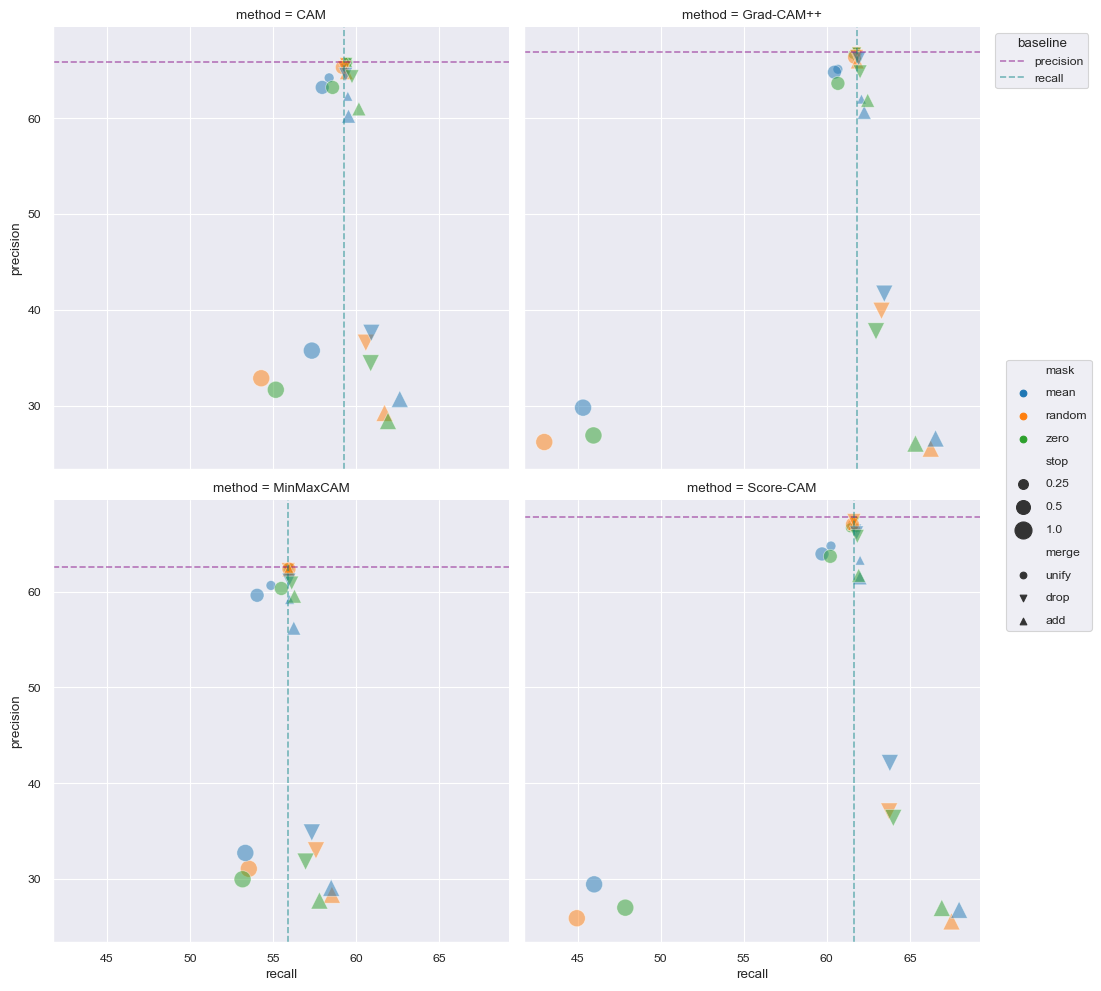
\includegraphics[width=0.99\textwidth]{fig_iter_mask_cam_resnet50_syn_d4b.png}
    \caption[Score map based iterative localization performance for ResNet-50 on synthetic dataset d4b]{Score map based iterative localization performance for ResNet-50 on synthetic dataset d4b. The cross-hair lines mark the best precision and recall for non-iterative localization.}
    \caption*{Source: Author}
    \label{fig:prec_iter_mask_cam_resnet50_syn_d4b}
    \end{center}
\end{figure}

\subsection{Evaluation for ResNet-50 on ImageNet dataset}
Here we evaluate the results of oracle-based and score map based iterative localization using CAM-based methods for the ResNet-50 network on the ImageNet validation dataset. The CAM-based methods used are CAM, Grad-CAM++, Score-CAM and MinMaxCAM. The former three methods are evaluated on a model trained without regularization while the latter is evaluated on a model trained with MinMaxCAM regularization. Due to time constraints, we were unable to evaluate score map based iterative localization for Score-CAM.

\subsubsection{Oracle-based iterative localization}

The results of the iterative localization methods for the ResNet-50 network, evaluated on the ImageNet validation dataset, are shown in Figure \ref{fig:prec_iter_resnet50_imagenet}. The best performing methods are those that are positioned closest to the upper right corner of the plot. Observing the plots for all localization methods, we can see two distinct groups: One group that improves recall at the cost of decreasing precision, and another group that performs worse for both precision and recall when compared to the baseline.

\begin{figure}[h]
    \begin{center}       
    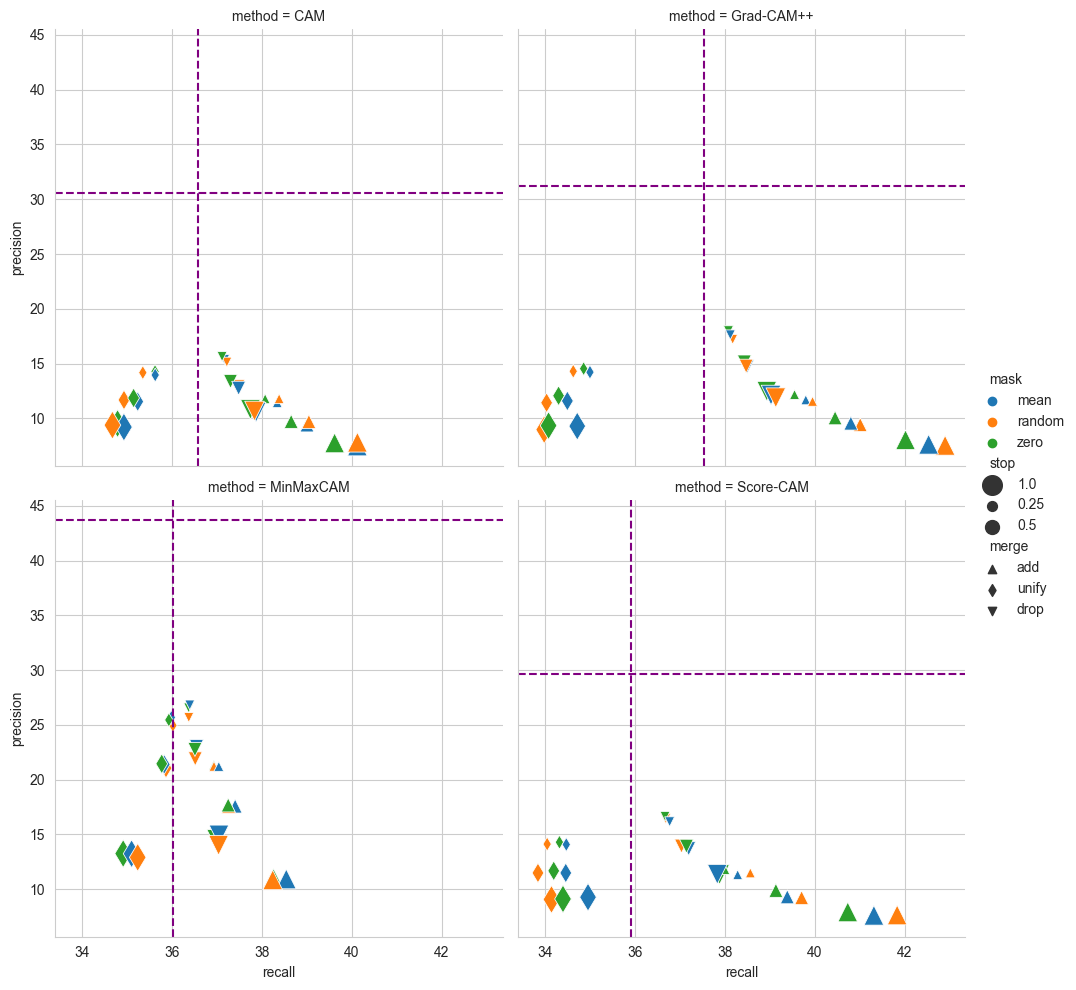
\includegraphics[width=0.99\textwidth]{fig_iter_resnet50_imagenet.png}
    \caption[Oracle-based iterative localization performance for ResNet-50 on ImageNet dataset]{Oracle-based iterative localization performance for ResNet-50 on ImageNet dataset. The cross-hair lines mark the best precision and recall for non-iterative localization.}
    \caption*{Source: Author}
    \label{fig:prec_iter_resnet50_imagenet}
    \end{center}
\end{figure}

The first group consists of the methods that apply as merge strategy either 'drop' or 'add', where the 'add' strategy gives a substantially higher gain in recall, but at a higher drop in precision. In this group, there is an almost linear relationship between precision and recall and the applied classification score drop threshold for a certain merge strategy. In the second group are the iterative localization methods that apply a unify merge strategy. Intuitively, unifying predicted bounding boxes from previous iterations with newly predicted bounding boxes increases the risk generating larger but few bounding boxes, and thus impacting both precision and recall.

\subsubsection{Score map based iterative localization}

For score map based iterative localization we evaluated the same CAM-based methods as oracle based localization for ResNet-50 on the ImageNet. Figure \ref{fig:prec_iter_mask_bbox_vs_camresnet50_imagenet} shows the comparison of results for both iterative localization approaches. The results are plotted such that, for a specific CAM-based method, we can make a column-wise comparison between the oracle approach (top row) and score map approach (bottom row).

For both approaches we can observe for each CAM-based method that the more recall is improved, the higher the loss in precision. We see this trend for all bounding box merge strategies, except the 'unify' merge strategy. In the latter case, both precision and recall are worse than the non-iterative baseline.

For score map based iterative localization, a much higher gain in recall is achieved for the 'add' merge strategy, than for the oracle based approach. 


\begin{figure}[h]
    \begin{center}       
    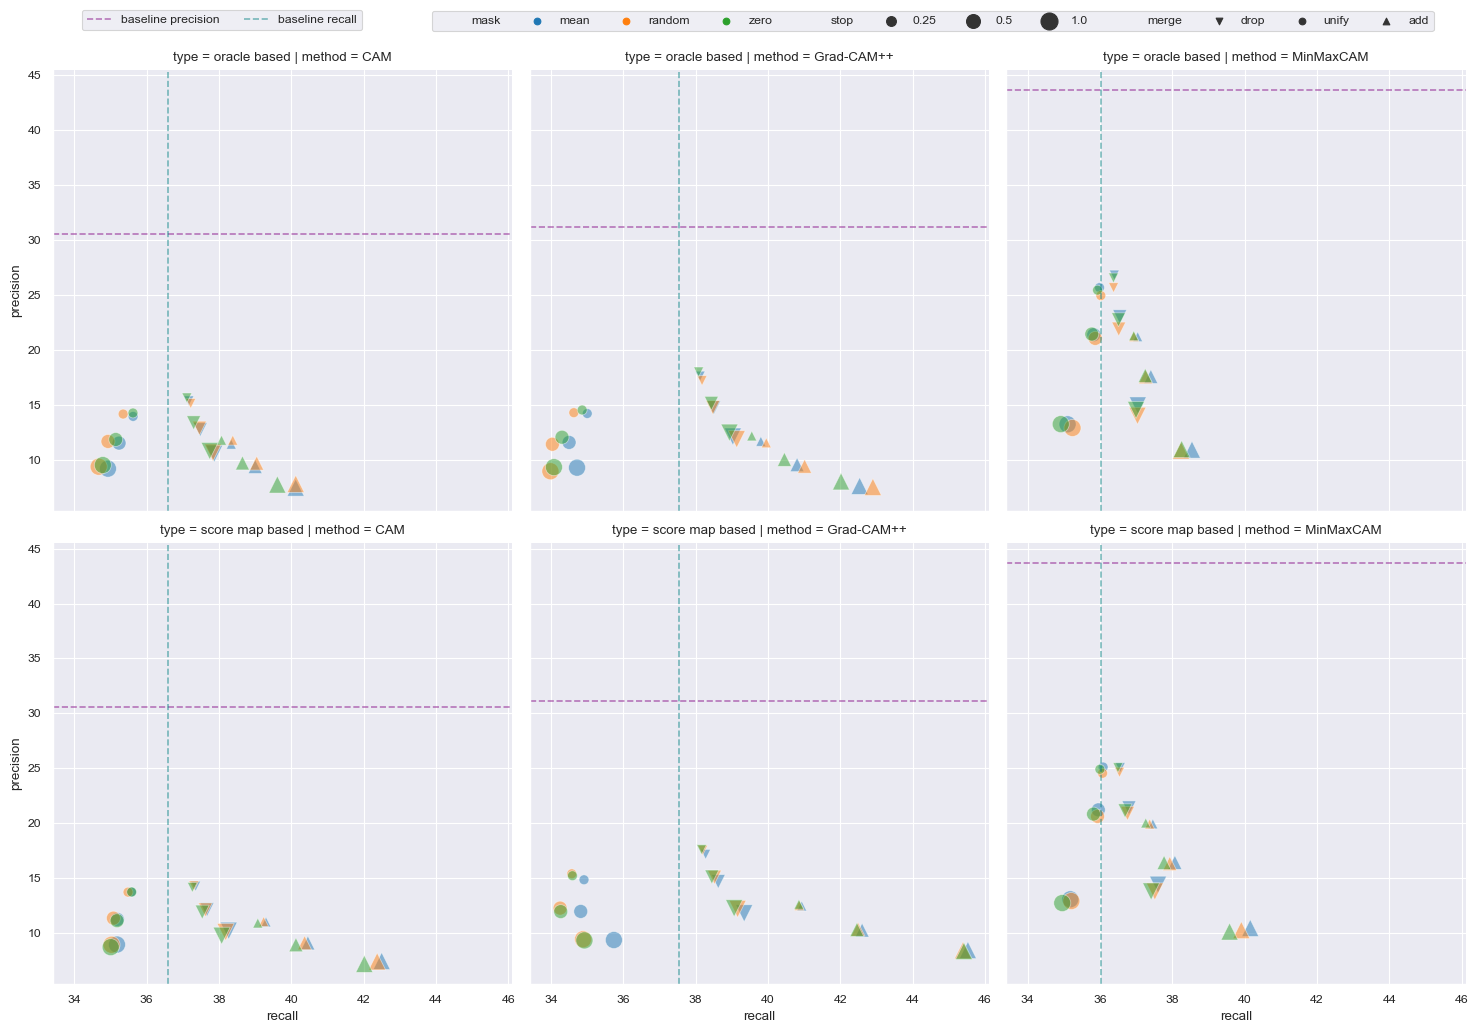
\includegraphics[width=0.99\textwidth]{fig_iter_mask_bbox_vs_cam_resnet50_imagenet.png}
    \caption[Oracle versus score map based iterative localization performance for ResNet-50 on ImageNet dataset]{Oracle (top row) versus score map (bottom row) based iterative localization performance using CAM (left), Grad-CAM++ (middle) and MinMaxAM (right) for ResNet-50 on ImageNet dataset. The cross-hair lines mark the best precision and recall for non-iterative localization.}
    \caption*{Source: Author}
    \label{fig:prec_iter_mask_bbox_vs_camresnet50_imagenet}
    \end{center}
\end{figure}